
\documentclass[oneside,a4paper]{book}
%\pagestyle{headings}


%=============================================================================

\usepackage{amsthm}
\usepackage{xspace}
\usepackage{float}
\usepackage{ifthen}
\usepackage{amsbsy}
\usepackage{amssymb}
\usepackage{balance}
\usepackage{booktabs}
\usepackage{graphicx}
\usepackage{rotating}
\usepackage{multirow}
\usepackage{needspace}
\usepackage{microtype}
\usepackage{bold-extra}
\usepackage{geometry}
\usepackage{varioref}
\usepackage{xcolor}
\usepackage{textcomp}
\usepackage{listings}
\usepackage[normalem]{ulem} %emphasize still italic
\usepackage{ucs}
\usepackage{booktabs}

% \usepackage[utf8]{inputenc}
% \usepackage[htt]{hyphenat}
\usepackage{times}
\usepackage{url}
\usepackage{alltt}
\usepackage{amsmath}
\usepackage{xfrac}
\usepackage{subfigure}
\usepackage{appendix}
\usepackage{stmaryrd}   % for the \shortuparrow
\usepackage[utopia]{quotchap}

\usepackage{setspace}
\usepackage[numbers, sort&compress]{natbib}
\usepackage{mdwlist}        % support for better spaced lists
% allows for temporary adjustment of side margins
\usepackage{chngpage}
\usepackage[normalem]{ulem} 

% constants

\newcounter{qcounter}

% commands
\newcommand{\n}{$\cdot$}
\newcommand{\y}{\checkmark}
\newcommand{\subscript}[1]{$_{\textrm{\footnotesize{#1}}}$}
\newcommand{\superscript}[1]{$^{\textrm{\footnotesize{#1}}}$}
\newcommand{\vertical}[1]{\raisebox{-4em}{\begin{sideways}{#1}\end{sideways}}}

\newboolean{showedits}
\setboolean{showedits}{true} % toggle to show or hide edits
\ifthenelse{\boolean{showedits}}
{
       \newcommand{\ugh}[1]{\textcolor{red}{\uwave{#1}}} % please rephrase
       \newcommand{\ins}[1]{\textcolor{blue}{\uline{#1}}} % please insert
       \newcommand{\del}[1]{\textcolor{red}{\sout{#1}}} % please delete
       \newcommand{\chg}[2]{\textcolor{red}{\sout{#1}}{\ra}\textcolor{blue}{\uline{#2}}} % please change
}{
       \newcommand{\ugh}[1]{#1} % please rephrase
       \newcommand{\ins}[1]{#1} % please insert
       \newcommand{\del}[1]{} % please delete
       \newcommand{\chg}[2]{#2}
}


% ============================================================================
% Put edit comments in a really ugly standout display

\usepackage{xcolor}
\usepackage[normalem]{ulem}
\newcommand{\ra}{$\rightarrow$}


% comments \nb{label}{color}{text}
\newboolean{showcomments}
\setboolean{showcomments}{true}
\ifthenelse{\boolean{showcomments}}
    {\newcommand{\nb}[3]{
        {\colorbox{#2}{\bfseries\sffamily\scriptsize\textcolor{white}{#1}}}
        {\textcolor{#2}{\sf\small$\blacktriangleright$\textit{#3}$\blacktriangleleft$}}}
     \newcommand{\version}{\emph{\scriptsize$-$Id$-$}}
%	 \newcommand{\ugh}[1]{\textcolor{red}{\uwave{#1}}} % please rephrase
%	 \newcommand{\ins}[1]{\textcolor{blue}{\uline{#1}}} % please insert
%	 \newcommand{\del}[1]{\textcolor{red}{\sout{#1}}} % please delete
%	 \newcommand{\chg}[2]{\textcolor{red}{\sout{#1}}{\ra}\textcolor{blue}{\uline{#2}}} % please change
	 \newcommand{\chk}[1]{\textcolor{ForestGreen}{#1}} % changed, please check
	}
    {\newcommand{\nb}[3]{}
     \newcommand{\version}{}
	\newcommand{\chk}[1]{} % changed, please check
	}

% ============================================================================
% Make quotes be italic
\renewenvironment{quote}
    {\list{}{\rightmargin\leftmargin}%
     \item\relax\begin{it}}
    {\end{it}\endlist}

\newcommand{\ttimes}{\ensuremath{\times}}

%=============================================================================

\newcommand{\needlines}[1]{\Needspace{#1\baselineskip}}

% source code
\usepackage{xcolor}
\usepackage{textcomp}
\usepackage{listings}
\definecolor{source}{gray}{0.9}
\lstset{
	language={},
	% characters
	tabsize=3,
	upquote=true,
	escapechar={!},
	keepspaces=true,
	breaklines=false,
	alsoletter={:},
	breakautoindent=true,
	columns=fullflexible,
	showstringspaces=false,
	basicstyle=\footnotesize\ttfamily,
	% background
	frame=single,
    framerule=0pt,
	backgroundcolor=\color{source},
	% numbering
	numbersep=5pt,
	numberstyle=\tiny,
	numberfirstline=true,
	% captioning
	captionpos=b,
	numberbychapter=false,
	% formatting (html)
	moredelim=[is][\textbf]{<b>}{</b>},
	moredelim=[is][\textit]{<i>}{</i>},
	moredelim=[is][\uline]{<u>}{</u>}}
\newcommand{\ct}{\lstinline[backgroundcolor=\color{white},basicstyle=\footnotesize\ttfamily]}
\newcommand{\lct}[1]{{\small\tt #1}}


%----------------------------------------------------------------------------
% references
\newcommand{\tabref}[1]{\hyperref[{tab:#1}]{Table~\ref*{tab:#1}}}
\newcommand{\figref}[1]{\hyperref[{fig:#1}]{Figure~\ref*{fig:#1}}}
\newcommand{\secref}[1]{\hyperref[{sec:#1}]{Section~\ref*{sec:#1}}}
\newcommand{\lstref}[1]{\hyperref[{lst:#1}]{Listing~\ref*{lst:#1}}}
\newcommand{\charef}[1]{\hyperref[{cha:#1}]{Chapter~\ref*{cha:#1}}}
%----------------------------------------------------------------------------

% abbreviations
\tracingcolors 4
\setcounter{tocdepth}{3}
\setcounter{secnumdepth}{3}
\newcommand{\ie}{\emph{i.e.,}\xspace}
\newcommand{\eg}{\emph{e.g.,}\xspace}
\newcommand{\etc}{\emph{etc.}\xspace}
\newcommand{\etal}{\emph{et al.}\xspace}


\newcommand{\newevenside}{
	\ifthenelse{\isodd{\thepage}}{\newpage}{
	\newpage
        \phantom{placeholder} % doesn't appear on page
	\thispagestyle{empty} % if want no header/footer
	\newpage
	}
}

\def\stretchfactor{1}
\newcommand{\mychapter}[1]{\setstretch{1}
    \chapter{#1}\setstretch{\stretchfactor}}

%----------------------------------------------------------------------------
\newcommand{\lessSpace}{\vspace{-1em}}
\DeclareGraphicsExtensions{.pdf,.png}
\graphicspath{{images/}}
\newcommand{\fig}[4]{
	\begin{figure}[#1]
		\centering
		\includegraphics[width=#2\textwidth]{#3}
		\lessSpace
		\caption{\label{fig:#3}#4}
	\end{figure}}

% ===========================================================================


\newcommand{\thesistitle}{Automating high-quality translations for Mobile Apps}
\newcommand{\thesisauthor}{Wanzenried \& Stefan}
\newcommand{\thesisleiter}{Prof. Dr. Philippe Cudr\'{e}-Mauroux}
\newcommand{\thesisasst}{Roman Prokofyev}
\newcommand{\thesissubtitle}{}
\newcommand{\thesisdate}{May 2016}



% ===========================================================================

\usepackage[ colorlinks=true, urlcolor=black, linkcolor=black,
			citecolor=black, bookmarksnumbered=true, bookmarks=true,
			plainpages=false,
			pdftitle={\thesistitle}, pdfauthor={\thesisauthor},
			pdfsubject={\thesissubtitle}, pdfpagelabels]{hyperref}

\newcommand{\hrref}[2]{\hyperref}
% ===========================================================================
% ===========================================================================


% D O C U M E N T
% % % % % % % % % % % % % % % % % % % % % % % % % % % % % % % % % %
\begin{document}

% T I T L E
% % % % % % % % % % % % % % % % % % % % % % % % % % % % % % % % % %
\begin{titlepage}  
  \begin{center}  
  
  \begin{figure}[t]  
  \vspace*{-2cm}        % to move header logo at the top 
  \center{
\includegraphics[scale=0.2]{logos/MSc_quer.png}}
  \vspace{0.4in}     
  \end{figure}

    \thispagestyle{empty}
    
    {\bfseries\Huge \thesistitle \par
    \Large \vspace{0.1in} \thesissubtitle \par}

    \vspace{0.3in} 
    \LARGE{\textbf{Master Thesis} \\}
    \vspace{0.4in}

    {\Large \thesisauthor \par from \par Bern BE, Switzerland}
    
    \vspace{0.3in}
%    {\Large Home University \par}
    {\Large Philosophisch-naturwissenschaftliche Fakult\"{a}t \\
            der Universit\"{a}t Bern \par}
    \vfill
    {\Large \thesisdate \par}
    \vspace{0.3in}
    %Leiter der Arbeit: \par
%   {\Large \thesisleiter, Research Group, Institute, University, Supervisor}\par
   {\Large \thesisleiter, eXascale Infolab, University of Fribourg, Switzerland, Supervisor}\par
   {\Large \thesisasst, eXascale Infolab, University of Fribourg, Switzerland, Assistant}
  

  \vspace{0.9in}
 
  % === Logos ==============================================     
  \begin{figure}[htp]
    \centering
    
\includegraphics[scale=0.30]{logos/UNI_Bern.png}\hfill
    
\includegraphics[scale=0.30]{logos/UNI_Neuenburg.png}\hfill
    
\includegraphics[scale=0.80]{logos/UNI_Fribourg.png}
  \end{figure}
  % === // Logos ===========================================    


  \end{center}

\end{titlepage}


% A B S T R A C T
% % % % % % % % % % % % % % % % % % % % % % % % % % % % % % % % % %
\chapter*{\centering Abstract}
\begin{quotation}
\noindent 
Every day, hundreds of mobile applications are added to stores such as Google Play or AppStore. Many of them are intended to be used internationally, and thus require translation of the interface. At the same time, many more mobile apps are already available for download in these stores. By leveraging the translation bases of existing applications, we could immediately provide high-quality translations for new apps without need to go through a human-translation process. 

This project aims to extract and parse translations of existing applications to see if they can be used to translate new ones. A prototype web application allows to translate a mobile application from a given source to a target language. Translations are generated using models based on Statistical Machine Translation techniques. Finally, the quality of the produced translations is evaluated and compared between the different models.
\end{quotation}
\clearpage



\chapter*{\centering Acknowledgements}
\begin{quotation}
\noindent 
First and foremost, I would like to thank Roman Prokofyev and
Professor Philippe Cudr\'{e}-Mauroux, who proposed the project and supervised my work, for their excellent support throughout this thesis. Without their advice and ideas, this thesis would not have been possible.
\end{quotation}
\clearpage


% C O N T E N T S 
% % % % % % % % % % % % % % % % % % % % % % % % % % % % % % % % % % % % % % % %
\tableofcontents

\listoffigures

\listoftables

%%%%%%%%%%%%%%%%%%%%%%%%%%%%%%%%%%
%%%% NEW CHAPTER %%%%%%%%%%%%%%%%%%%%%
%%%%%%%%%%%%%%%%%%%%%%%%%%%%%%%%%%
\chapter{Introduction}
\label{cha:introduction}

Android, iPhone and Windows smart phones are available in countries all over the world. If an app is intended to be used internationally, translating it into multiple languages can be important to attract users. Users may only understand and use the app if its text is available in their native language. Offering multiple languages is therefore crucial for paid apps to increase sales. However, translating an app requires additional effort. From a developer's perspective, all strings must be isolated in order to replace them with different values for each supported language. Furthermore, translating text itself is a difficult task which usually requires the work of a professional translator.

The main idea of this thesis is to collect translation data of existing apps and use them to translate new ones. Apps belonging to the same category share similar words or sentences. Also, sentences in mobile apps are typically short and thus easier to translate than longer, more complex sentences in books or news. Based on these facts, we argue that a Statistical Machine Translation (SMT) model could be used to automatically generate high-quality translations for mobile apps. 

To reduce the scope of different mobile operating systems and languages, we focus on automatic translations of Android apps from English to French and German. From now on, the term \emph{app} in this thesis refers to an Android application. French and German are chosen as target languages for the translations because they are natively spoken in Switzerland, which makes understanding the produced results easier.

SMT is the dominant approach in automating translations and used by services such as \emph{Google Translate}\footnote{\url{https://translate.google.com} (accessed: 16 May 2016)} and Microsoft's \emph{Bing Translator}\footnote{\url{https://www.bing.com/translator} (accessed: 16 May 2016)}. In this thesis, we use different SMT models and compare their results for translating mobile apps, both manually and automatically. A prototype web application is built, offering a common interface to translate strings or apps using the implemented translation systems.

\chapter{Problem Analysis}
\label{cha:problem_analysis}

This chapter first describes the importance of app localization. Next, we analyze what translation services are already available for this task. Finally, we briefly introduce SMT and explain how it can be used for the purpose of app translation.

%This chapter answers the question why it is an absolute must to localize mobile apps nowadays. We analyze what kind of services exist to translate apps. %Lastly, we identify the challenges we most likely will face during this project.%

\section{Importance of Translating Mobile Apps}

%https://web.archive.org/web/20150402231142/http://www.distimo.com/blog/2012_10_publication-the-impact-of-app-translations/%

%https://web.archive.org/web/20150327084808/http://www.distimo.com/publications%

Google encourages developers to localize their apps as per their localization checklist\footnote{\url{http://developer.android.com/distribute/tools/localization-checklist.html} (accessed: 16 May 2016)}:

\begin{quote}
Android and Google Play offer you a worldwide audience for your apps, with an addressable user base that's growing very rapidly in countries such as Japan, Korea, India, Brazil, and Russia. We strongly encourage you to localize as it can maximize your apps’ distribution potential resulting in ratings from users around the world.
\end{quote}
The developer should first identify the countries where the app will be distributed based on the overall market size and opportunity, app category, local pricing, etc. According to the identified countries, the supported languages are determined. Ideally an app supports multiple languages already before the first version is available on the app store. Users may install the app only once and forget about it, if they are not able to understand it.

Since 2013, Google offers an app translation service~\citep{website_google_translation_service}. Several developers who participated at the pilot program shared their results after translating their apps:

\begin{itemize}
\item The developers of the game \emph{Zombie Ragdoll}\footnote{\url{https://play.google.com/store/apps/details?id=com.rvappstudios.zombieragdoll} (accessed 12 May 2016)} used this tool to launch their new game simultaneously in 20 languages in August 2013. When they combined app translation with local marketing campaigns, they found that 80\% of their installs came from non-English-language users~\citep{website_google_translation_service}.
\item Dating app \emph{SayHi}\footnote{\url{https://play.google.com/store/apps/details?id=com.unearby.sayhi} (accessed 12 May 2016)} expanded into 13 additional languages using the app translation service. They saw 120\% install growth in localized markets and improved user reviews of the professionally translated UI~\citep{website_google_translation_service}.
\item The developer of card game \emph{G4A Indian Rummy}\footnote{\url{https://play.google.com/store/apps/details?id=org.games4all.android.games.indianrummy.prod} (accessed 12 May 2016)} found that the app translation service was easier to use than their previous translation methods, and saw a 300\% increase with user engagement in localized apps~\citep{website_google_translation_service}.
\end{itemize}

In 2012, company \emph{App Annie}\footnote{\url{https://www.appannie.com} (accessed 12 May 2016)} (former called \emph{Distimo}), published a study where they analyzed the impact of translations to iPhone apps~\citep{website_impact_of_translations_to_mobile_apps}. They found out that the use of native language is still limited in several countries, including Italy, Russia and Brazil. Native-only apps are mostly used in Asian countries (see Figure~\ref{fig:problem_analysis_impact_languages}).\ugh{the message of last two sentences in unclear, please change.}
The study followed 200 iPhone apps that introduced native language support in a market and observed their growth. One week after the local language support was introduced with an app update, download rate increased by 128\% and revenue by 26\%.

%Another case-study by David Janner from make app magazine\footnote{\url{http://makeappmag.com/iphone-app-localization-keywords}} observed the impact of translating one single app.
%

\begin{figure}[H]
    \centering
    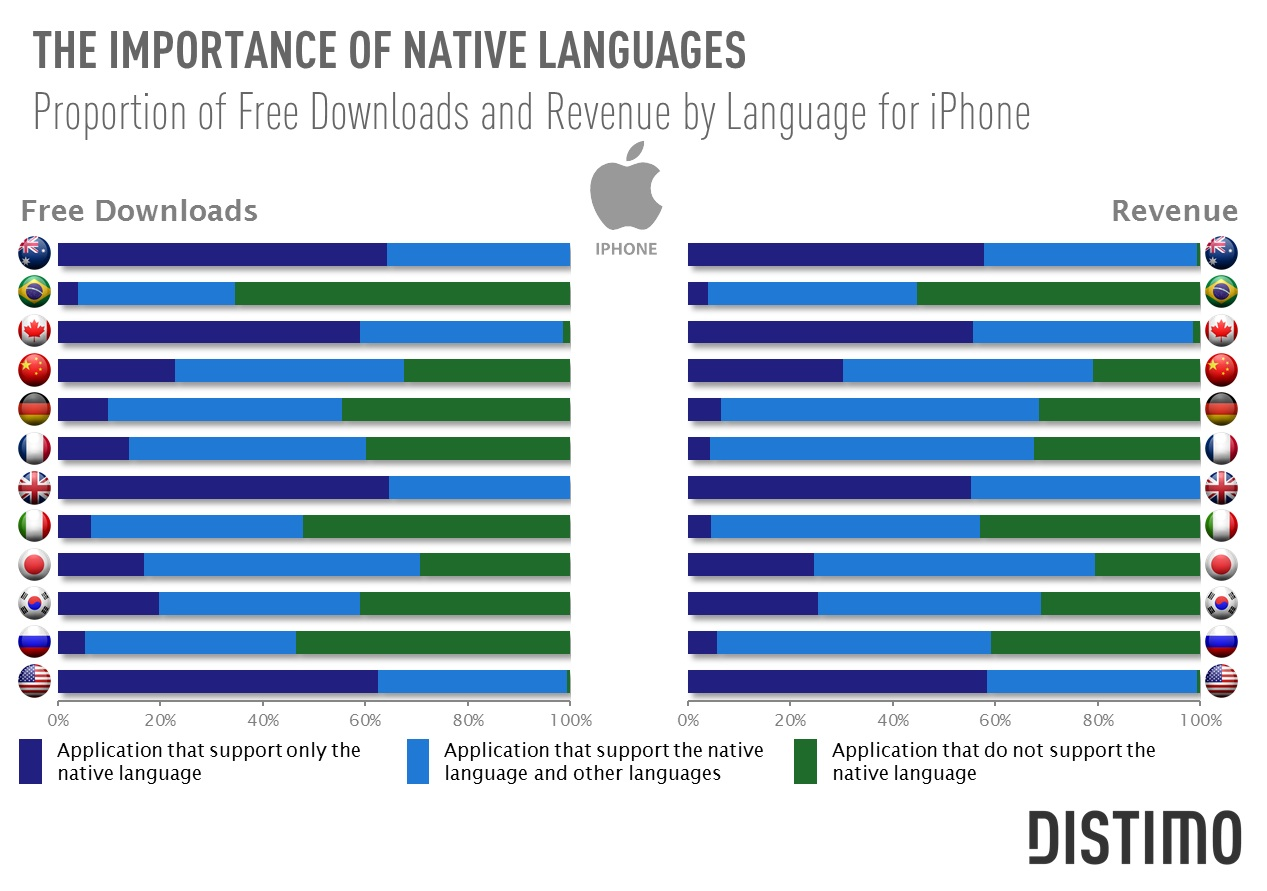
\includegraphics[width=0.9\textwidth]{images/problem_analysis_app_annie.jpg}
    \caption[Proportion of free downloads and revenue of iPhone apps by language \cite{website_impact_of_translations_to_mobile_apps}]{Graphic from \citep{website_impact_of_translations_to_mobile_apps} showing the proportion of free downloads and revenue of iPhone apps by language.}
    \label{fig:problem_analysis_impact_languages}
\end{figure}
Besides offering a better user experience by translating apps, both examples show that proper localization also directly impacts the number of downloads and revenue. 

\section{Translation Services}

Most of the existing services employ human translator in order to guarantee translation quality, including Google's app translation service~\citep{website_google_translation_service}. The developer can choose from third-party vendors who are entitles by Google to offer high-quality translations. According to Google, the costs range from \$75 to \$150 depending on the app size.

Another possibility to translate apps quickly is to use Crowdsourcing. Here, we ask people in a crowdsourcing platform to do the translations for us. \ugh{Try to formulate sentences in the same style, e.g., Crowdsoucing platforms allow people to perform various tasks, including ... } This approach is often used in combination with machine translation: Initial translations are produced with machine translation, which are then improved or corrected by human translators. Facebook used crowdsourcing to translate their website: ``In March 2008, through crowdsourcing, the entire site was translated into French within 24 hours by allegedly over 4,000 native French speakers.''\footnote{\url{https://en.wikipedia.org/wiki/Crowdsourcing_as_Human-Machine_Translation} (accessed 12 May 2016)}. Examples of crowdsourcing translation platforms are \emph{Translation Cloud}\footnote{\url{http://www.translationcloud.net/} (accessed 13 May 2016)} and \emph{Gengo}\footnote{\url{http://gengo.com/} (accessed 13 May 2016)}. Using these platforms, people who are fluent in at least two languages can earn money by translating or correcting strings. To avoid cheaters, an initial language proficiency test must be passed.

Translation services that based solely on machine translations do not seem to exist. However, developers could use existing translation APIs to produce translations. Popular providers are Microsoft\footnote{\url{http://datamarket.azure.com/dataset/bing/microsofttranslator} (accessed 12 May 2016)} and Google\footnote{\url{https://cloud.google.com/translate/docs/} (accessed 12 May 2016)}. Microsoft's translation service offers a free plan which is limited to translate 2 million characters per month. Paid plans also exist, where the amount of characters is increased, 32 million characters cost \$300 per month. The translation API from Google does not offer any free plan but the pricing model is different: One pays \$20 per 1 million characters of text.

% http://www.translationcloud.net/
% https://www.microsoft.com/en-us/translator/getstarted.aspx
% http://datamarket.azure.com/dataset/bing/microsofttranslator

\section{Statistical Machine Translation}

``Machine translation has a long history, but over the last decade or two, its evolution has taken on a new direction - a direction that is mirrored in other subfields of natural language processing. This new direction is grounded in the premise that language is so rich and complex that it could never be fully analyzed and distilled into a set of rules, which are then encoded into a computer program. Instead, the new direction is to develop a machine that discovers the rules of translation automatically from a large corpus of translated text, by pairing the input and output of the translation process, and learning from the statistics over the data.'' \cite{smt_book_koehn}

As SMT is the dominant approach in machine translation, it is consequential to use it for our purpose of translating mobile apps. In machine translation literature, the SMT models are usually trained on a large parallel corpus, for example the \emph{European Parliament Proceedings Parallel Corpus} \cite{website_parallel_corpus}. This corpus consists of many sentences for a given language pair, e.g. EN-FR holds over 2 million sentences. Our corpus will hold the extracted sentences from existing apps. We expect to collect less but shorter sentences.

To automatically evaluate the quality of machine produced text, a metric called \emph{BLEU} \citep{bleu_score} is mostly used. We adapt this procedure and also use BLEU to evaluate our translations in Chapter \ref{cha:evaluation}. %In our context, we train the We use two different SMT algorithm (see Chapter \ref{cha:related_work}) and analyze how they perform in the context of translating short sentences of mobile apps.

%There exists a recurring translation task of the \emph{Workshop on %statistical machine translation}, which focuses on translating %European language pairs by improving existing systems%\footnote{\url{http://www.statmt.org/wmt15/translation-task.html}}.

%In this thesis, we compare two different SMT algorithm and evaluate %how they perform in the context of translating short sentences of %mobile apps. The models are therefore applied on a much smaller data %set than usual.

%\section{Challenges}
%
%
%\begin{itemize}
%\item Quality of translations: Bad translation of existing apps have a direct impact on the quality of our produced translations. While we can assume that popular apps are properly translated, this might not be true for smaller, free apps.
%\item Where and how to obtain large amount of apps? Google doesn't offer a way to download multiple apps at once. Downloading apps on a mobile device one after another is a time consuming task.
%\item Server Hardware: Training translation models with a large amount of data requires a solid server with a fast CPU and enough memory.
%\end{itemize}


\chapter{Related Work}
\label{cha:related_work}
%In which we learn what have other done to address similar problems. For example, the work of Star \cite{Star89}

%Overview of SMT
%Has been done but not specific domain of short sentences mobile

This chapter explains the theory of two popular models in SMT . The first one is called \emph{Statistical Phrase-Based Translation} and was introduced in 2003 \cite{smt_phrase_based}. The second, more recent model, uses \emph{Deep Learning Neural Networks} to perform translations \cite{smt_deep_learning1, smt_deep_learning}.

\section{Phrase-Based Machine Translation}
\label{sec:phrase_based_mt}
\subsection{Model}

Given the task to translate a sentence from a foreign language \(f = f_1, f_2, f_3..., f_m\) into an english sentence \(e = e_1, e_2, e_3 ..., e_n\), the translation model is based on conditional probability:

\[P(e|f)\]
To find the best english translation \(e_{best}\), the following equation is used (Bayes rule).

\[e_{best} = argmax_eP(e|f)\]
\[= argmax_e\frac{P(f|e)P(e)}{P(f)}\]
\[= argmax_e P(e|f)P(e)\]
where \(P(e)\) is called the \emph{language model}\footnote{\url{https://en.wikipedia.org/wiki/Language_model} (accessed: 17 May 2016)} and \(P(f|e)\) is the \emph{translation model}.
\\
\\
The translation model is further decomposed:

\[p(\bar{f}_1^I|\bar{e}_1^I) = \prod_{i=1}^I \phi(\bar{f}_i^I|\bar{e}_i^I) d(start_i - end_{i-1} -1)\]
where \(\phi\) is called the \emph{phrase translation probability} and \(d\) is the \emph{reordering probability}.
The foreign sentence \emph{f} is broken up into \emph{I} phrases \(\bar{f}_i\). Each foreign phrase is translated into an English phrase \(\bar{e}_i\).

Reordering is handled by a \emph{distance based reordering model}. We define \(start_i\) as the position of the first word of the foreign input phrase that translates to the \emph{i}th English phrase, and \(end_i\) as the position of the last word of that foreign phrase. The reordering distance is the number of words skipped when taking foreign words out of sequence (see figure \ref{fig:related_work_phrase_based_reordering}) \citep{smt_book_koehn}.

\begin{figure}[H]
    \centering
    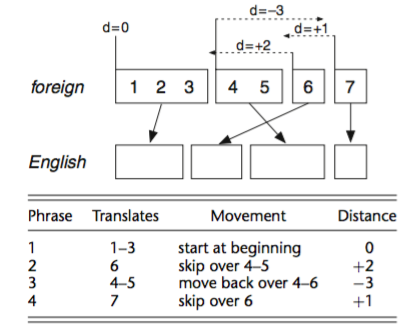
\includegraphics[width=0.4\textwidth]{images/related_work_phrase_based_reordering.png}
    \caption{Distance based reordering \cite{smt_book_koehn}}
    \label{fig:related_work_phrase_based_reordering}
\end{figure}

\emph{d} is turned into a proper probability distribution by applying an exponentially decaying cost function \(d(x) = \alpha^{|x|}\) with \(\alpha \epsilon [0,1]\). This means that movements of phrases over large distances are more expensive than shorter movements or no movement at all \citep{smt_book_koehn}.


\subsection{Learning a Phrase Translation Table}

Building a phrase translation table involves three stages:
\begin{enumerate}
\item \textbf{Word alignment} The words of each sentence from the parallel corpus of the foreign and English language must be aligned in order to extract phrase pairs. The alignment is typically done by using one of the IBM models\footnote{\url{https://en.wikipedia.org/wiki/IBM_alignment_models} (accessed 13 May 2016)}. Figure \ref{fig:related_work_word_alignment} shows an example of word alignment for a top translation from our corpus.
\item \textbf{Extraciton of phrase pairs} Extract all phrase pairs of parallel sentences that are consistent with word alignment. A phrase pair (\(\bar{f}\),\(\bar{e}\)) is consistent with an alignment \emph{A}, if all words \(f_1,...,f_n\) in \(\bar{f}\) that have alignment points in \emph{A} have these with words \(e_1,...,e_n\) in \(\bar{e}\) and vice versa \citep{smt_book_koehn}.
\item \textbf{Scoring phrase pairs} Assign probabilities to phrase translations.
\end{enumerate}

\begin{figure}[H]
    \centering
    
\includegraphics[width=0.4\textwidth]{images/related_work_word_alignment.png}
    \caption{Word alignment between a top sentence of the parallel English-French corpus.}
    \label{fig:related_work_word_alignment}
\end{figure}

\begin{figure}[H]
    \centering
    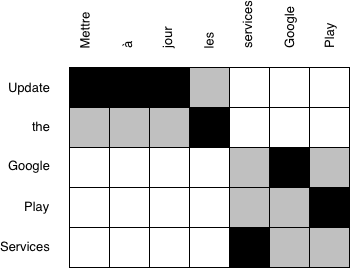
\includegraphics[width=0.4 \textwidth]{images/related_work_phrase_alignment.png}
    \caption{Extraction of phrase pairs consistent with word alignment}
    \label{fig:related_work_phrase_alignment}
\end{figure}


We are able to extract the following phrase pairs from the example sentence (phrases marked with an * match the extractions from Figure \ref{fig:related_work_phrase_alignment}):
\begin{itemize}
\item Update the Google Play Services / Mettre \a`a jour les services Google Play
\item Update / Mettre \a`a jour
\item Update the / Mettre \a`a jour les *
\item Google Play Services / services Google Play *
\item The Google Play Services / les services Google Play
\item Google Play / Google Play
\item Google / Google
\item Play / Play
\item Services / services
\item the / les
\end{itemize}
The last step is to estimate the phrase translation probabilities by  relative frequency:

\[\phi(\bar{f}|\bar{e}) = \frac{count(\bar{e},\bar{f})}{\sum_{\bar{f}_i }count(\bar{e},\bar{f}_i)}\]
These probabilities are put in the phrase translation table together with the foreign phrases (see Figure \ref{fig:phrase_table_example}).

\begin{table}[H]
\centering
\begin{tabular}{@{}lr@{}}
\toprule
Foreign Phrase & \(\phi(\bar{f}|\bar{e})\)  \\ \midrule
param\a`etres     & 0.9         \\
r\a'eglages       & 0.36        \\
configuration  & 0.15        \\ \bottomrule
\end{tabular}
\caption[Example of a phrase translation table]{Example of a phrase translation table containing the estimated probabilities for translating the English word ``Settings'' to French.}
\label{fig:phrase_table_example}
\end{table}


\subsection{Decoding}
\label{sec:phrase_based_decoding}

Decoding is the process of finding a translation for a given input sentence. 
%Due to the big size of a phrase translation table, the search method is heuristic based. This means that the search algorithm can't explore the entire search space and therefore there is no guarantee that it will return the best translation.%
Recall the model to compute the translation probability:

\[e_{best} = argmax_{e} \prod_{i=1}^I \phi(\bar{f}_i|\bar{e}_i) d(start_i - end_{i-1} -1) p_{LM}(e)\]

\begin{itemize}
\item \textbf{Phrase translation} Pick phrase \(\bar{f}_i\) to be translated as phrase \(\bar{e}_i\) by looking up the score from the phrase translation table.
\item \textbf{Reordering} The previous phrase ended in \(end_{i-1}\), the current phrase starts at \(start_i\). Compute \(d(start_i - end_{i-1} -1)\)
\item \textbf{Language model} For a \emph{n}-gram model, we need to keep track of the last \(n - 1\) words. The score is computed for every added word \(w_i\): \(p_{LM}(w_i|w_i - (n-1), ..., w_{i-1})\)
\end{itemize}
The algorithm reads the input sentence from left to right and creates a new hypothesis by picking any phrase translation at a time. The score is computed incrementally for each partial hypothesis. This is repeated recursively until all hypotheses have been expanded. A hypothesis covering all input words cannot be expanded further and forms an end point in the search graph (Figure \ref{fig:related_work_hypothesis}). To get the best translation, we pick the completed hypothesis with the highest probability score and backtrack through the search graph \citep{smt_book_koehn}. 

\begin{figure}[H]
    \centering
    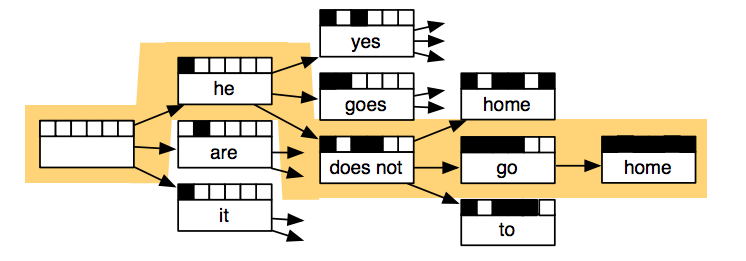
\includegraphics[width=0.7\textwidth]{images/related_work_hypothesis.png}
    \caption[Decoding process \cite{smt_book_koehn}]{Hypothesis expanded by translating the German sentence ``er geht ja nicht nach hause'' to English. The squares on top indicate a coverage vector of translated German words (filled black if covered) \cite{smt_book_koehn}.}
    \label{fig:related_work_hypothesis}
\end{figure}
This process creates an exponential number of hypothesis. To reduce the search space, the following methods are applied:

\begin{itemize}
\item \textbf{Recombination} Two hypothesis paths lead to two matching hypotheses, e.g. have the same English words in the output. The worse hypothesis is dropped.
\item \textbf{Stack Pruning} Bad hypotheses are removed early. Hypothesis that have translated the same number of input words are put into a stack, so that they are comparable. The number of hypotheses in a stack is limited, for example by keeping only \emph{k} hypotheses according to a score. This score is typically a combination of the partial probability score and a future cost estimation for translating the remaining sentence.
\end{itemize}


\section{Deep Learning Neural Networks}
\label{sec:related_work_deep_learning}
Translating with neural networks is based on a encoder-decoder architecture \cite{smt_deep_learning1, smt_deep_learning}. Two \emph{recurrent neural networks} (RNN)\footnote{\url{https://en.wikipedia.org/wiki/Recurrent_neural_network} (accessed: 13 May 2016)} are involved: The first RNN encodes a variable-length sequence into a fixed-length vector representation. The second RNN decodes a given fixed-length vector back into a variable-length sequence.
We first describe shortly the working of a RNN before explaining the encoder-decoder architecture in more detail. 

%Beside the papers, we also want to mention a blog post\footnote{\url{https://devblogs.nvidia.com/parallelforall/introduction-neural-machine-translation-with-gpus/}} by NVIDIA which offers a very detailed explanation of the model.%


\subsection{Recurrent Neural Network}

A recurrent neural network is a class of artificial neural network where connections between units form a directed cycle. It consists of a hidden state \(h\) and an optional output \(y\) which operates on a variable-length sequence \( x = (x_1, ..., x_n)\). At each time step \(t\), the hidden state \(h_{t}\) is updated by:

\[  h_{t} = f(h_{t-1}, x_t) \]
where \(f\) is a non-linear activation function. The function described in \cite{smt_deep_learning1} is motivated by a \emph{long short-term memory (LSTM)} unit\footnote{\url{https://en.wikipedia.org/wiki/Long_short-term_memory} (accessed 13 May 2016)}, but much simpler to compute and implement.

A RNN can learn a probability distribution over a sequence by being trained to predict the next symbol in a sequence. In this case, the output at each timestep \(t\) is the conditional distribution \( p(x_t | x_{t-1}, ... , x_1) \).


\subsection{Encoder}

The encoder RNN reads each word of the source sentence sequentially in the form of a \emph{One-hot vector}. This binary vector has the size of the vocabulary and zeros everywhere except a \(1\) at the position corresponding to the index of the word in the source vocabulary.

The internal state \(h_t\) changes each time a new word is read:

\[  h_{t} = f(h_{t-1}, x_t) \]
At the end of processing each word, the hidden state of the RNN is a summary \(c\) of the source sentence (see Figure \ref{fig:related_work_encoder}). 

\begin{figure}[H]
    \centering
    
\includegraphics[width=0.85\textwidth]{images/related_work_encoder.png}
    \caption[Overview of the Encoder RNN]{Encoder RNN: The final hidden state (marked bold) contains the summary vector.}
    \label{fig:related_work_encoder}
\end{figure}
It is very interesting how the summary vector \(c\) looks like. In  \cite{smt_deep_learning} they projected multiple summary vectors to the two-dimensional space (see Figure \ref{fig:related_work_summary_vector}). The plot shows that similar sentences are close together in the summary vector space.

\begin{figure}[H]
    \centering
    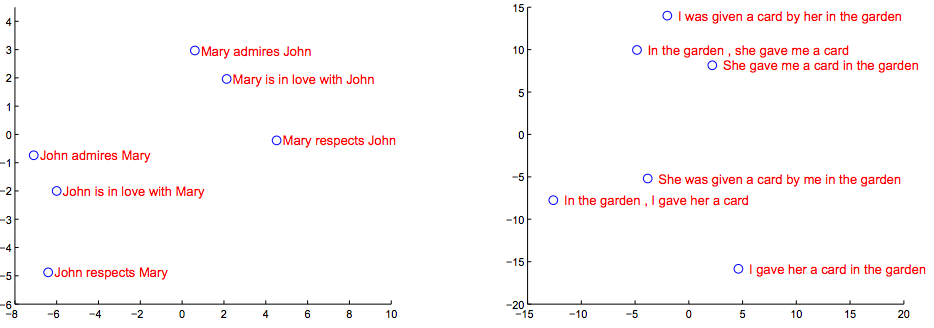
\includegraphics[width=0.95\textwidth]{images/related_work_pca_summary_vector.png}
    \caption[Summary vectors projected to the two-dimensional space \cite{smt_deep_learning}]{Summary vectors from multiple sentences. Similar sentences in terms of syntax and semantics are grouped together \cite{smt_deep_learning}.}
    \label{fig:related_work_summary_vector}
\end{figure}


\subsection{Decoder}

The decoder is another RNN which is trained to generate the output sentence by predicting the next word \(y_t\) given the hidden state \(h_t\). Both \(y_t\) and \(h_t\) are conditioned on \(y_{t-1}\) and the summary vector \(c\) given from the encoder RNN. The hidden state of the decoder is computed by

\[  h_t = f(h_{t-1}, y_{t-1}, c) \]
The conditional distribution of the next target word is

\[ P(y_t|y_{t-1},y_{t-2},...,y_1,c) = g(h_t, y_{t-1}, c) \]
for given activation functions \(f\) and \(g\). The latter must produce valid probabilities.

\subsection{Training}

The proposed encoder-decoder system is trained by maximizing the \emph{log-likelihood}\footnote{\url{https://en.wikipedia.org/wiki/Likelihood_function} (accessed: 13 May 2016)} of the training corpus. Training requires a parallel corpus \(C\) of source and target sentences \((X^n, Y^n)\). The sentences are represented as sequence of one-hot vectors. We can compute the conditional log-probability of \(Y^n\) given \(X^n\) by \( log P(Y^n|X^n, \theta) \). The log-likelihood of the training corpus is written as:

\[ L(C,\theta) = \frac{1}{N} \sum_{n=1}^N log P(Y^n|X^n, \theta) \]
where \(N\) is the number of training samples and \(\theta\) is the set of model parameters.
Maximizing the log-likelihood function can be done by using \emph{stochastic gradient descent}\footnote{\url{https://en.wikipedia.org/wiki/Stochastic_gradient_descent} (accessed: 13 May 2016)}.

\chapter{Data Analysis}
\label{cha:data_analysis}

\section{Apps}

A total of 698 free Android apps were collected from various categories\footnote{Click on Categories to see a list of available categories at:  \url{https://play.google.com/store/apps?hl=en} (accessed: 13 May 2016)}, ensuring a good mix of different translations. Figure \ref{fig:data_analysis_top_apps_en} shows the top ten apps according to the number of available English translations. Note that the counts indicate the number of effective translations after eliminating uninteresting data during pre-processing the corpus (see Chapter \ref{cha:data_extraction_prep_storage}). Most of the apps have similar counts for all the three languages. Surprisingly, some apps provide more translations for German and French than English. Different counts can happen because of:

\begin{enumerate}
\item Not all strings need to be translated, some English words remain the same in the target language e.g. ``E-Mail''.
\item Android stores the translations key-value based in one XML file per language. These files could be out of sync, the developer either forgot to add or remove a French/German translation.
\item Some translations were abandoned during pre-processing.
\end{enumerate}
34 apps did not isolate their strings in XML files, we assume that they are hardcoded in the programming code. This leaves an effective number of 664 apps where we could extract translations. However, 241 apps among them were not multilingual and therefore not useful for building translation systems. Unfortunately, apps are not marked as multi-language in the app store, so we only know if there are isolated translations available after downloading and extracting the data.

\begin{figure}[H]
    \centering
    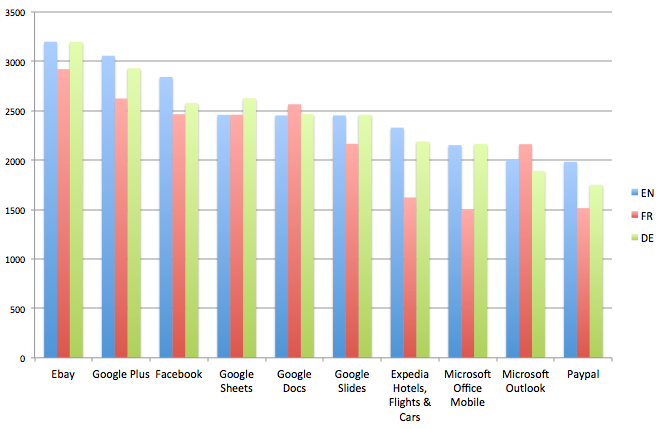
\includegraphics[width=1.0\textwidth]{images/data_analysis_top_apps_en.png}
    \caption{Top apps by the number of English translations}
    \label{fig:data_analysis_top_apps_en}
\end{figure}


\section{Languages}

We collected a total of 423 multilingual apps, offering its content for at least two languages. Figure \ref{fig:data_analysis_n_langs} shows the number of apps for the ten most used languages. French and German, where we focus on this thesis, are both in the top four. The top apps are translated in many more languages. Overall, 117 different languages were available.

\begin{figure}[H]
    \centering
    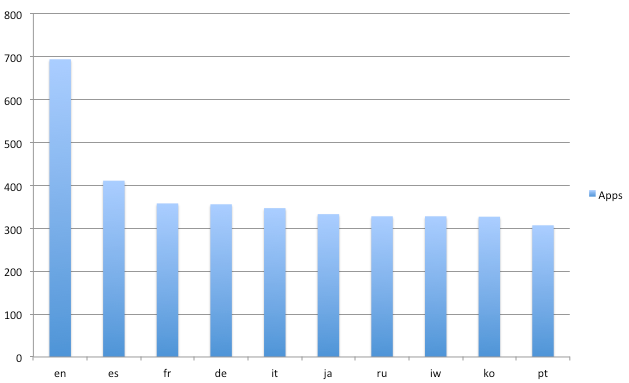
\includegraphics[width=1.0\textwidth]{images/data_analysis_languages_count.png}
    \caption{Number of apps available in the top ten languages.}
    \label{fig:data_analysis_n_langs}
\end{figure}


\section{Extracted Sentences}

This sections covers statistics regarding the extracted sentences per language, including the top sentences, top \(n\)-grams and sentence lengths. Note that the term \emph{sentence} in this section describes single words, sentences or multiple sentences, separated by punctuation.

In total, we collected 114'947 parallel sentences for the English-French language pair and 114'773 for English-German, respectively. The monolingual data holds 187'642 English sentences, 126'883 French sentences and 126'975 German sentences. Again, the counts are measured after pre-processing the extracted data (see Section \ref{sec:preprocess_translations}).


\subsection{Top Sentences}

\begin{table}[H]
\centering
\resizebox{\textwidth}{!}{%
\begin{tabular}{@{}llllllll@{}}
\toprule
EN & Count &  & FR & Count &  & DE & Count \\ \midrule
Cancel & 1894 &  & Annuler & 1067 &  & Abbrechen & 886 \\
Done & 1230 &  & Supprimer & 745 &  & Google Play-Dienste aktivieren & 730 \\
Settings & 1102 &  & Connexion & 745 &  & Google Play-Dienste installieren & 728 \\
Search & 884 &  & Mettre \`{a} jour & 486 &  & Anmelden & 664 \\
Delete & 704 &  & Rechercher & 485 &  & L\"{o}schen & 664 \\
Enable Google Play services & 692 &  & Param\`{e}tres & 450 &  & Aktualisieren & 652 \\
Get Google Play services & 690 &  & Mettre \`{a} jour les services Google Play & 370 &  & Einstellungen & 569 \\
Log Out & 556 &  & Activer services google Play & 368 &  & Fertig & 548 \\
Update & 545 &  & Activer les services Google Play & 366 &  & Weiter & 484 \\
Share & 541 &  & Installer les services Google Play & 366 &  & Schliessen & 428 \\ \bottomrule
\end{tabular}
}
\caption{Top ten sentences for English, French and German}
\label{table:data_analysis_top_terms}
\end{table}

One can see that all three languages share similar top sentences, although they do not perfectly align.

%\subsection{Number of Sentences}%
%
%\begin{table}[H]
%\centering
%\begin{minipage}{0.48\textwidth}
%\centering
%\begin{tabular}{@{}ll@{}}
%\toprule
%DE-EN  & EN-FR  \\ \midrule
%114'773 & 114'947 \\ \bottomrule
%\end{tabular}
%\caption{Parallel data}
%\label{my-label}
%\end{minipage}
%\hfill
%\begin{minipage}{0.48\textwidth}
%\centering
%\begin{tabular}{@{}lll@{}}
%\toprule
%EN     & FR     & DE     \\ \midrule
%18'7642 & 12'6883 & 12'6975 \\ \bottomrule
%\end{tabular}
%\caption{Monolingual data}
%\label{my-label}
%end{minipage}
%\end{table}
%Both language pairs contain a similar amount of parallel sentences. The %monolingual corpus contains more English sentences than German and F%rench.


\subsection{Sentence Lengths}

As expected, most sentences are very short and consist of less than 5 words for all languages. %The longest sentence from the English corpus has 9632 words. 
The lengths were measured on the monolingual corpus after tokenization, which means that punctuation is also included in the counts.


\begin{figure}[H]
    \centering
    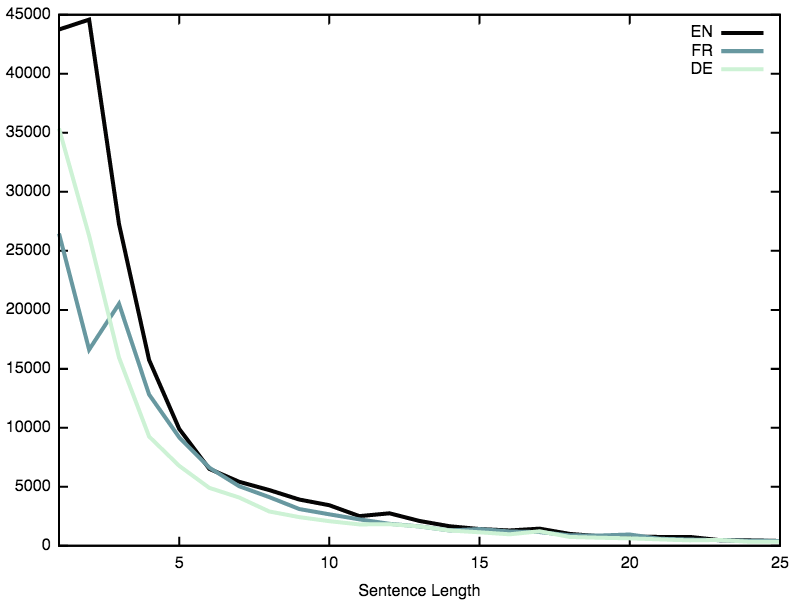
\includegraphics[width=1.0\textwidth]{images/data_analysis_sentences_count.png}
    \caption{Length of sentences for English, French and German}
    \label{fig:data_analysis_languages_count}
\end{figure}
\subsection{N-Grams}

\begin{table}[H]
\centering
\begin{tabular}{@{}llllll@{}}
\toprule
EN     & Count & FR     & Count & DE     & Count \\ \midrule
to     & 28160 & de     & 32818 & Sie    & 14383 \\
the    & 19306 & \`{a}      & 13094 & nicht  & 8216  \\
your   & 14238 & la     & 10956 & die    & 7853  \\
you    & 11144 & le     & 10701 & und    & 7366  \\
and    & 9962  & les    & 10619 & zu     & 5791  \\
a      & 9657  & pour   & 8057  & der    & 5783  \\
in     & 8338  & votre  & 7674  & auf    & 5575  \\
is     & 8087  & des    & 7090  & ist    & 5447  \\
this   & 7522  & et     & 7025  & werden & 5337  \\
of     & 7340  & pas    & 6976  & von    & 5329  \\
 \bottomrule
\end{tabular}
\caption{Top unigrams from the monolingual corpus}
\label{my-label}
\end{table}


\begin{table}[H]
\centering
\begin{tabular}{@{}llllll@{}}
\toprule
EN            & Count & FR                 & Count & DE                     & Count \\ \midrule
Google Play   & 3348  & Google Play        & 3366  & Google PlayDienste     & 2639  \\
Play services & 2807  & de la              & 2915  & Sie die                & 1458  \\
try again     & 2270  & services Google    & 2905  & Sie es                 & 1183  \\
to the        & 1705  & \`{a} jour             & 2353  & Sie sich               & 975   \\
want to       & 1647  & les services       & 1762  & versuchen Sie          & 835   \\
you want      & 1484  & que vous           & 1593  & kann nicht             & 806   \\
will be       & 1359  & de votre           & 1373  & konnte nicht           & 795   \\
Please try    & 1328  & de passe           & 1303  & es erneut              & 714   \\
of the        & 1325  & Impossible de      & 1284  & auf Ihrem              & 667   \\
is not        & 1258  & a \'{e}t\'{e}              & 1027  & in der                 & 667   \\
\bottomrule
\end{tabular}
\caption{Top bigrams from the monolingual corpus}
\label{my-label}
\end{table}


\begin{table}[H]
\centering
\begin{tabular}{@{}llllll@{}}
\toprule
EN                   & Count & FR                          & Count & DE                               & Count \\ \midrule
Google Play services & 2805  & services Google Play        & 2889  & versuchen Sie es                 & 804   \\
you want to          & 1407  & les services Google         & 1714  & Google PlayDienste aktivieren    & 565   \\
Please try again     & 1187  & mot de passe                & 920   & Sie es erneut                    & 465   \\
try again later      & 794   & ne fonctionnera pas         & 877   & sind Google PlayDienste          & 452   \\
Are you sure         & 740   & ne sont pas                 & 832   & Google PlayDienste erforderlich  & 445   \\
This app wont        & 686   & Cette application ne        & 713   & Bitte versuchen Sie              & 427   \\
you sure you         & 630   & application ne fonctionnera & 712   & PlayDienste erforderlich die     & 417   \\
sure you want        & 596   & Mettre \`{a} jour               & 620   & Google PlayDienste installieren  & 396   \\
and try again        & 579   & mise \`{a} jour                 & 571   & Google PlayDienste aktualisieren & 396   \\
can not be           & 555   & Google Play qui             & 480   & Sie es sp\"{a}ter                    & 394   \\ \bottomrule
\end{tabular}
\caption{Top trigrams from the monolingual corpus}
\label{my-label}
\end{table}

\chapter{Data Extraction, Preparation and Storage}
\label{cha:data_extraction_prep_storage}

\section{Extract Translations}

An Android app has the form of a single binary file (suffix .apk). The XML files containing the translations are packed inside the .apk file. We used a software called \emph{Apktool}\footnote{\url{http://ibotpeaches.github.io/Apktool/} (accessed: 13 May 2016)} to reverse engineer existing apps and extract the needed XML files.

\begin{figure}[H]
    \centering
    
\includegraphics[width=0.6\textwidth]{images/data_extraction_xml.png}
    \caption[Storage of translation strings in XML files]{For each language, the translations are stored in a XML file}
    \label{fig:data_extraction_xml}
\end{figure}
Inside the \texttt{strings.xml} files, translations are stored key-value based. Each string has a unique key which holds the translation value for each language. Here is an example how an English XML file looks like, followed by its German counterpart:

\lstset{
language=XML,
morekeywords={encoding,resources,string }
}
\begin{lstlisting}
<?xml version="1.0" encoding="utf-8"?>
<resources>
    <string name="close_app">Close</string>
    <string name="back">Back</string>
    ...
</resources>
\end{lstlisting}

\lstset{
language=XML,
morekeywords={encoding,resources,string }
}
\begin{lstlisting}
<?xml version="1.0" encoding="utf-8"?>
<resources>
    <string name="close_app">Schliessen</string>
    <string name="back">Zurück</string>
    ...
</resources>
\end{lstlisting}

\section{Preprocess Translations}
\label{sec:preprocess_translations}
This task involves two parts. First of all, the translations are sanitized from unwanted information such as HTML tags. Some strings are omitted at this stage because they do not provide any meaningful value to the translation process, for example URLs. Secondly, the sanitized strings are tokenized so that they can be used to train a SMT system.

\subsection{Sanitizing}

The following rules are used to get rid of unwanted translations or parts of it:

\begin{itemize}
\item Trim the string from newlines (\texttt{\textbackslash n}), tabs (\textbackslash t) or carriage returns (\textbackslash r)
\item Strip any HTML tags
\item Omit strings that are URLs (starting with http or www)
\item Remove strings placeholders like \texttt{\%s} or \texttt{\%1\$s}
\item Ignore words with less than 3 characters
\item Finally, the resulting string is trimmed again from spaces and must contain at least one alphanumerical character
\end{itemize}


\subsection{Tokenization and Truecasing}

Tokenization is required to separate words from punctuation. Each token is separated by a space character: ``\texttt{Hi, my name is John.}'' becomes ``\texttt{Hi , my name is John .}''

After tokenizsation, \emph{truecasing}\footnote{\url{https://en.wikipedia.org/wiki/Truecasing} (accessed: 13 May 2016)} was applied to the text corpus. In contrast to lowercasing, truecasing determines the proper capitalization of words. This is done by first analyzing how words are mostly capitalized. The proper case is then applied to each word. It is especially useful for words starting a sentence, that are written uppercase in many languages. For example the word ``This'' starting a sentence will become ``this'', because it is usually written lowercase.


\section{Data storage}


\subsection{Parallel and Monolingual Corpus}

After pre-processing the translations, they are written to text files, one sentence per line. The corpus is split into parallel and monolingual data. A parallel corpus (often also called bitext) describes sentence aligned text-files of one language pair. All sentences must be aligned so that line \(x\) of the first language corresponds to line \(x\) of the second language. In order to get a random mix of translations from different apps, the sentences are shuffled before they are written to the files. The parallel corpus can be used by any SMT system to train the models. If the model requires a separate development set of parallel sentences, we can split the existing corpus at any percentage, e.g. use 80\% as training data and the remaining 20\% as development set.
In addition, data of each language is also stored monolingual. All sentences of one language are written into a single text file. This is for example used to build language models, which are an important part of a phrase-based translation model (see Chapter \ref{sec:phrase_based_mt}).

The data analysis (see Chapter \ref{cha:data_analysis}) showed that the monolingual corpus holds more sentences than the parallel corpus for all three languages. The reason is that the XML files are not synchronized perfectly: If an English sentence, identified by the translation key, is missing in French or German, it cannot be part of the parallel corpus.

\subsection{Apache Solr}
\label{sec:apache_solr}

We needed a simple way to store all translations, preferably with additional meta data, to perform data analysis and calculate statistics.
\emph{Apache Solr}\footnote{\url{http://lucene.apache.org/solr/} (accessed: 13 May 2016)} is used for this purpose. Solr is an open source text search platform built on top of \emph{Apache Lucene}. It allows to store the translations with additional meta data, such as the translation key and a unique app ID. Due to its way of indexing text data, Solr is very fast when querying for translation strings. Furthermore, built in tools allow us to get nice statistics, for example the top translations grouped by language.

Solr is also used as \emph{Baseline Translation System}, where we translate strings with a simple algorithm directly from the collected data in Solr (see Chapter \ref{cha:translation_process_baseline}).

\subsubsection{Setup and Schema}

Solr offers so called \emph{cores} where each core manages a separate index, schema and configuration\footnote{\url{https://cwiki.apache.org/confluence/display/solr/Solr+Cores+and+solr.xml} (accessed: 13 May 2016)}. In our setup we created one core per language and one document per translation string. The schema is identical for each core (language) and consists of the following fields:

\begin{itemize}
\item \textbf{id} Unique ID used by Solr to identify a document.
\item \textbf{app\_id} Each app must have a unique app-ID.
\item \textbf{key} The translation key from the XML file.
\item \textbf{value} The translation value (word or sentence) corresponding to the above key.
\item \textbf{value\_lc} Again the translation value, additionally indexed with a special start- and ending delimiter. This allows us to search for exact values of any translation string.
\end{itemize}

\begin{figure}[H]
    \centering
    
\includegraphics[width=0.8\textwidth]{images/data_extraction_solr_schema.png}
    \caption[Storage of translation data in Solr]{Translations are stored in a document inside a separate core per language}
    \label{fig:data_extraction_solr_schema}
\end{figure}

The data in the \texttt{value} and \texttt{value\_lc} fields is stored tokenized and lowercased. The Solr \emph{Standard Tokenizer}\footnote{\url{https://cwiki.apache.org/confluence/display/solr/Tokenizers\#Tokenizers-StandardTokenizer} (accessed: 13 May 2016)} splits text into tokens, treating whitespace and punctuation as delimiters. Delimiter characters are discarded.

\subsubsection{Queries}

Solr offers a REST based interface to query the database. There is also a built in web application which allows to inspect results.
Here is an example query where we search for the string ``Log Out'' in the English core\footnote{You must be connected to the LAN of the University of Fribourg in order to access the referenced domain. Also note that the parameters should be fully url-encoded, this was omitted in this report for better readability.}. The maximum amount of results is set to 500 rows and the return type is JSON:
\\
\\
\url{http://diufpc114.unifr.ch:8983/solr/en/select?q=value:"Log\%20Out"&rows=500&wt=json&indent=true}
\\
\\
This query finds a total of 458 results (see Listing \ref{lst:solr_json_response}). There are not only exact matches returned, the term ``Log Out'' can occur as substring in a longer sentence. By default, Solr does not offer the possibility to return only exact matches. However, we can simulate this behaviour with the help of the \texttt{value\_lc} field, which indexed the translation value together with a special start- and end delimiter (\texttt{SOLR\_S} and \texttt{SOLR\_E}):
\\
\\
\url{http://diufpc114.unifr.ch:8983/solr/en/select?q=value_lc:"SOLR_S\%20Log Out\%20SOLR_E"&rows=500&wt=json&indent=true}
\\
\\
This query returns only 396 results, representing exact matches. Note that the case of the search term doesn't matter and whitespace and punctuation are ignored. Executing the above query with the term ``log Out .'' returns the same results. This behaviour is especially useful when looking up translations, as we don't need to worry about proper case or punctuation.

\begin{minipage}{\linewidth}
\begin{lstlisting}[caption=JSON response from Solr, label=lst:solr_json_response]
"response": {
    "numFound": 458,
    "start": 0,
    "docs": [
      {
        "id": "com.flaregames.gargoyles_com_facebook_loginview_log_out_action",
        "app_id": "com.flaregames.gargoyles",
        "key": "com_facebook_loginview_log_out_action",
        "value": "Log Out",
        "value_lc": "SOLR_S Log Out SOLR_E"
      },
      {
        "id": "com.instagram.android_must_log_out_one_click_login",
        "app_id": "com.instagram.android",
        "key": "must_log_out_one_click_login",
        "value": "You must log out in order to login using this link.",
        "value_lc": "SOLR_S You must log out in order to login using this link. SOLR_E"
      },      ...
      ]
}
\end{lstlisting}
\end{minipage}

\chapter{Translation Process}
\label{cha:translation_process}

This chapter describes different translation systems that were used to translate apps. We first introduce a simple \emph{Baseline System}, that translates sentences based on the available data in Solr. The next section focuses on \emph{Moses}, a phrase-based SMT system. Lastly, \emph{Tensorflow} was used to provide translations with deep neural networks. The latter two implement closely the models introduced in Chapter \ref{cha:related_work}.

%The ``Baseline System'' makes direct use of the data stored in Solr and produces translations with a simple algorithm. The second system, ``Moses''\footnote{Moses SMT system: \url{http://www.statmt.org/moses/}}, is a open source phrase-based SMT software. Lastly ``Tensorflow''\footnote{Tensorflow: \url{https://www.tensorflow.org/}} was used to produce translations with the help of deep learning neural networks. Tensorflow is a software library for machine intelligence, recently released as open source by Google.%

\section{Baseline System}
\label{cha:translation_process_baseline}

The \emph{Baseline System} makes direct use of the data stored in Solr and produces translations with a simple algorithm. Remember how the data is organized in Solr (see section \ref{sec:apache_solr}): Each translation is stored in a document with a fixed schema and each document belongs to one core. To lookup a translation, the following procedure is used:

\begin{enumerate}
\item Lookup the string to translate in the core of the source language.
\item Parse the result documents and extract the \texttt{app\_id} and \texttt{key} fields.
\item Lookup translations in the target language by querying the target core with the collected \texttt{app\_id}s and \texttt{key}s.
\item Count the number of unique translations found. The best translation is the value that was mostly used.
\end{enumerate}
Figure \ref{baseline_system_table_available_translations} shows an example for the available translations for the English word ``Settings''. The best translation according to the highest count among all apps is ``param\`{e}tres''.

\begin{table}[H]
\centering
\begin{tabular}{@{}lr@{}}
\toprule
Translation                                  & Count \\ \midrule
param\`{e}tres & 48    \\
r\'{e}glages                                     & 3     \\
settings                                     & 3     \\
configuration                                & 1     \\ \bottomrule
\end{tabular}
\caption{Available translations for ``Settings'' in French.}
\label{baseline_system_table_available_translations}
\end{table} 

\subsection{Algorithm}

Given a string \(S = [ \; s_1  \; s_2  \; ...  \; s_n \; ]\) with words \(s_i\) in the source language, we want to produce a string \(T = [ \; t_1 \; t_2  \; ... \; t_n \; ]\) in the target language. The algorithm recursively tries to translate the longest substrings of \(S\) by looking up translations for the substrings in Solr. This process is repeated until there are left only single words \(s_i\) to translate.

\begin{enumerate}
\item Check if we find any translation for \(S\) directly. If so, return the translation and exit.
\item Start translating the longest substrings of \(S\). To build the substrings, we move a ``window'' of size \(length(S) - i\) from left to right over \(S\), where \(i\) is the iteration level. Let \(length(S) = 7\); the following two  substrings of length 6 are possible at the first iteration (\(i = 1\)):

\begin{center}
\( V_1 = [ \; s_1 \; s_2 \; s_3 \; s_4 \; s_5 \; s_6 \; ] \; [ \; s_7 \; ]\)

\( V_2 = [ \; s_1 \; ] \; [ \; s_2 \; s_3 \; s_4 \; s_5 \; s_6 \; s_7 \; ]\)
\end{center}

Now, we search for translations for all substrings in both variations \(V_1\) and \(V_2\). If there are no translations available, the substring (window) size is reduced by one for the second iteration (\(i = 2\)):

\begin{center}

\(  V_1 = [ \; s_1 \; s_2 \; s_3 \; s_4 \; s_5 \; ] \; [ \; s_6 \; s_7 \; ]\)

\( V_2 = [ \; s_1 \; ] \; [ \; s_2 \; s_3 \; s_4 \; s_5 \; s_6 \; ] \; [ \; s_7 \; ]\)

\( V_3 = [ \; s_1 \; s_2 \; ] \; [ \; s_3 \; s_4 \; s_5 \; s_6 \; s_7 \; ]\)

\end{center}

This process of reducing the substring length is repeated until we can translate a substring of at least one variation \(V_j\).

\item Let's consider what happens if there are translations available. For each variation \(V_j\), we count the number of available translations for their substrings \(\bar{S}_i\). We continue with the variation \(\tilde{V}\) having the highest total count of translations among their substrings:

\[ \tilde{V} = argmax\sum_i count\_translations(\bar{S}_i) \]

If there is a translation available for each substring \(\bar{S}_i\) of \(\tilde{V}\), we can build the output string \(T\) directly by concatenating the substring translations: 

\begin{center}
\(T = \bar{T}_1 \; \bar{T}_2 \; \bar{T}_3 \; ... \; \bar{T}_n\)
\end{center}

Otherwise, we build the output string \(T\) incremental: If there is no translation found for substring \(\bar{S}_i\), we set \(S = \bar{S}_i\) and recursively call the algorithm again. If there are left single words to translate and no translation exists, we insert the source word into \(T\) by setting \(t_i = s_i\).

\end{enumerate}
This simple algorithm works well for translating short words or sentences where a direct translation exists in the target language. On the other hand, it suffers from the following problems if translating substrings is necessary:

\begin{itemize}
\item The sentences or words for the translated substrings are inserted at the same position in \(T\) where they occurred in the source string. This won't produce good results since words often need to be reordered depending on the target language.
\item Bad translations can have a direct impact on the result. For example, due to an error or uncompleted translation in the XML files, the English word ``the'' could be mapped to a sentence with many words.
\end{itemize} 


\subsection{Example}

Let us translate the source string ``Open the settings to change your username'' from English to French.

\begin{enumerate}
\item Check for a direct translation: No French translation available.
\item Start translating the substrings. The upper index indicates the number of translations found:

\begin{center}
\(V_1\) = [ Open the settings to change your ] \(^0\) [ username ] \(^{28}\)

\(V_2\) = [ Open ] \(^{63}\) [ the settings to change your username ] \(^0\)
\end{center}

Continue with Variation 2 since the count (63 + 0) is higher than the count from Variation 1 (0 + 28).

\item We set \(T\) = [ ouvrir ] and \(S\) = [ the settings to change your username ] and go recursive. Again, there does not exist a translation for \(S\) directly so the substrings are built:

\begin{center}
\(V_1\) = [ the settings to change your ] \(^0\) [ username ] \(^{28}\)

\(V_2\) = [ the ] \(^{1}\) [ settings to change your username ] \(^0\)
\end{center}

\item \(T\) = [ ouvrir ... nom d'utilisateur ] ; \(S\) = [ the settings to change your ]

\begin{center}
\(V_1\) = [ the settings to change ] \(^0\) [ your ] \(^{2}\)

\(V_2\) = [ the ] \(^{1}\) [ settings to change your ] \(^0\)
\end{center}

\item \(T\) = [ ouvrir ... votre nom d'utilisateur ] ; \(S\) = [ the settings to change ]

\begin{center}
\(V_1\) = [ the settings to ] \(^0\) [ change ] \(^{26}\)

\(V_2\) = [ the ] \(^{1}\) [ settings to change ] \(^0\)
\end{center}

\item \(T\) = [ ouvrir ... modifier votre nom d'utilisateur ] ; \(S\) = [ the settings to ]

\begin{center}
\(V_1\) = [ the settings ] \(^5\) [ to ] \(^{2}\)

\(V_2\) = [ the ] \(^{1}\) [ settings to ] \(^0\)
\end{center}

\item \(T\) = [ ouvrir les param\`{e}tres vers modifier votre nom d'utilisateur ] ; \(S\) = [ ] 

%\begin{center}
%\(V_1\) = [ the ] \(^1\) [ settings ] \(^{48}\)
%\end{center}


% \item \(T\) = [ ouvrir les param\`{e}tres vers modifier votre nom d'utilisateur ]

\end{enumerate}
At the last step, there are translations available for both substrings of \(V_1\) and the algorithm derived the following string: ``ouvrir les param\`{e}tres vers modifier votre nom d'utilisateur''


\section{Moses}

\emph{Moses}\footnote{\url{http://www.statmt.org/moses/} (accessed: 13 May 2016)} \cite{moses} is a open source SMT toolkit. The training process follows closely the phrase-based model described in section \ref{sec:phrase_based_mt}. The source code is available on \emph{GitHub}\footnote{\url{https://github.com/moses-smt/mosesdecoder} (accessed: 13 May 2016)}. This project is very active, there are frequent commits to the master branch by 72 contributors and documentation on their website is excellent.


\subsection{Training}

The training process requires sentence aligned parallel data to build the translation models, and monolingual data for the language models. We can make use of the sanitized and tokenized data as described in section \ref{sec:preprocess_translations}. The training process involves the following steps.

\begin{enumerate}
\item Build a language model from the monolingual data of the target language. Moses includes the \emph{KenLM toolkit}\footnote{\url{https://kheafield.com/code/kenlm/} (accessed 13 May 2016)} for this task.
\item Align words of the parallel sentences. We used an external library \emph{MGIZA}\footnote{\url{https://github.com/moses-smt/mgiza.git} (accessed: 13 May 2016)}, an extension of the popular \emph{GIZA++} word alignment toolkit \cite{giza_pp}. MGIZA is multi-threaded and runs faster on a multi-core machine.
\item Extract phrases: All phrases are dumped into one big file. The following listing shows some example content of this file. Each line contains: English phrase, French phrase and the alignment points of matching words (English-French).

\begin{lstlisting}[label=list:moses_phrase_extraction]
! as you can see from ||| ! comme vous pouvez le voir ||| 0-0 1-1 2-2 3-3 4-5
! as you can see ||| ! comme vous pouvez le voir ||| 0-0 1-1 2-2 3-3 4-5
! as you can ||| ! comme vous pouvez le ||| 0-0 1-1 2-2 3-3
! as you can ||| ! comme vous pouvez ||| 0-0 1-1 2-2 3-3
! as you ||| ! comme vous ||| 0-0 1-1 2-2
! as ||| ! comme ||| 0-0 1-1
\end{lstlisting}


\item Score phrases by computing the phrase translation probability \(\phi(\bar{f}|\bar{e})\) and build the phrase table. Here is an example how the content of the phrase table is organized in Moses for English-French:

\begin{lstlisting}[label=list:moses_phrase_table]
! your version of Google Play ||| ! votre version de Google Play ||| 1 0.04 1 0.22 
! your version of Google ||| ! votre version de Google ||| 1 0.04 1 0.24 
! your version of ||| ! votre version de ||| 1 0.0427528 1 0.245609 
! your version ||| ! votre version ||| 1 0.635219 1 0.508584 
! your ||| ! ton ||| 1 0.591003 0.0434783 0.00469507 
! your ||| ! votre ||| 1 0.794566 0.73913 0.542431
! your ||| ! your ||| 1 0.896708 0.130435 0.0173818
! your ||| . vos ||| 0.0416667 0.00483387 0.0434783 0.0112108
\end{lstlisting}

Each line contains the phrase pairs together with the computed phrase translations scores, in the following order:
\begin{enumerate}
\item Inverse phrase translation probability \(\phi(\bar{e}|\bar{f})\)
\item Inverse lexical weighting \(lex(\bar{e}|\bar{f})\)
\item Direct phrase translation probability \(\phi(\bar{f}|\bar{e})\)
\item Direct lexical weighting \(lex(\bar{f}|\bar{e})\)
\end{enumerate}

%Note that \(\bar{f}\) means ``foreign'' and \(\bar{e}\) stands for ``English''.

The \emph{lexical weighting} is an additional score to check the reliability of the phrase translation probability. Rare phrase pairs may cause problems if they are collected from noisy data. If both of the phrases \(\bar{f}\), \(\bar{e}\) only occur once in the training data, then \(\phi(\bar{f}|\bar{e}) = \phi(\bar{e}|\bar{f}) = 1\). This often overestimates how reliable rare phrase pairs are. Lexical weighting decomposes phrase pairs into its word translations, so that we can check how well they match up \citep{smt_book_koehn}.

\end{enumerate}
The output of the training process is the phrase translation table and a configuration file \texttt{moses.ini} containing all necessary configuration for the decoder to translate sentences.

Training one model, e.g. English-French with all parallel data only took about one hour. A more time consuming task is \emph{Tuning}, which is explained in the next section.

%Moses includes tools to binarise the pharse and reordering tables. The data is compiled into a format that can be quickly loaded.

\subsection{Tuning}
\label{subsec:moses_tuning}
Tuning refers to the process of finding the optimal weights for the linear translation model of Moses:

\[ p(e|f) = \phi(f|e)^{weight\_tm} LM(e)^{weight\_lm} D(e,f)^{weight\_dm} W(e)^{weight\_wp} \]
The probability cost that is assigned to a translation is a product of probability costs of four models:

\begin{itemize}
\item \(\phi(f|e)\) The \textbf{phrase translation table} ensures that the source and target phrases are good translations of each other.
\item \(LM(e)\) The \textbf{language model} ensures that the output of the target language is fluently.
\item \(D(e,f)\) The \textbf{distortion model} allows for reordering of the input sentence, but at a cost. The more reordering, the more expensive is the translation.
\item \(W(e)\) The \textbf{word penalty} ensures that the translations do not get too long or too short.
\end{itemize}
There is a weight assigned to each of these components that influences their importance. These weights can be passed to the decoder when translating sentences. The optimal weights depend on the languages and training corpus. However, Moses offers to optimize the weights automatically by maximizing the BLEU score \cite{bleu_score} on a small, separate set of parallel sentences (tuning set).

We used 80\% of the available parallel data for training and the remaining 20\% for tuning. Tuning takes much more time than training. Moses executes different tuning runs and measures the BLEU score achieved on the tuning set. The optimal weights were usually determined after 6-11 runs, which took about 3-6 hours.

\subsection{Decoding}

The decoder of Moses is controlled by the \texttt{moses.ini} file. This file stores the path to the phrase translation table and the language model. Additionally it also holds the tuned weights for the translation model. Many more configuration options\footnote{\url{http://www.statmt.org/moses/?n=Moses.DecoderParameters} (accessed 13. May 2016)} can be set in this file or passed as parameters when executing the decoder. Here is a summary from \cite{pdf_moses_manual} how the decoder of Moses works:

\begin{enumerate}
\item The decoder collects all phrase translations from the phrase table that could be applied on the input strings of words (translation options). The translation options are stored with the following information:
\begin{itemize}
\item First source word covered
\item Last source word covered
\item Phrase translation in the target language
\item Phrase translation probability
\end{itemize}
\item The output sentence is generated left to right in form of hypotheses. Each hypothesis is represented by:
\begin{itemize}
\item A link to the best previous state, so that we later can back track through the graph to find the best translation.
\item The cost (probability) and covered source words so far. A low cost means high probability.
\item An estimate of the future cost, how expensive it is to translate the remaining words of the source sentence.
\end{itemize}

The decoder uses \emph{Recombination} and a \emph{Beam Search} (see Section \ref{sec:phrase_based_decoding}) to reduce the size of the search space. 

%The beam search compares hypothesis covering the same number of source words in stacks. Given the cost so far and the future cost estimation, hypotheses that fall outside of the beam are pruned. The beam size can be defined by threshold and histogram pruning. A relative threshold cuts out a hypothesis with a probability less than a factor \(\alpha\) of the best hypotheses. Histogram pruning keeps a certain number \(n\) of hypotheses in each stack. 
\end{enumerate}
\textbf{Example} We translate the same example string as used in the previous chapter ``Open the settings to change your username'' to French. Here is the command to invoke the decoder:

\begin{lstlisting}[breaklines=true ]
echo 'Open the settings to change your username' | /home/stefan/mosesdecoder/bin/moses -f /home/stefan/AppTranslator/data/moses/en-fr/mert-work/moses.ini -verbose 3 &> moses_decoding.out 
\end{lstlisting}
We used histogram pruning with a stack size of 100 and the optimal model weights determined after tuning.

The decoder produces the following output string: ``ouvrir les param\`{e}tres pour modifier votre nom d' utilisateur''. Here are some statistics on how the decoder derived the target sentence:

\begin{itemize}
\item Total translation options collected: 197
\item Total hypotheses considered: 42614
\item Total hypotheses discarded: 31220
\item Total hypotheses recombined: 8292
\item Total hypotheses pruned: 2401
\end{itemize}

\section{Tensorflow}

\emph{Tensorflow}\footnote{\url{https://www.tensorflow.org/} (accessed: 13 May 2016)} is a software library for machine intelligence, open sourced by Google in November 2015. The source code is available on GitHub\footnote{\url{https://github.com/tensorflow/tensorflow} (accessed: 13 May 2016)} and the project is still under development.

Tensorflow includes a library to learn sequence to sequence models with neural networks. The implementation follows the encoder-decoder RNN model described in Section \ref{sec:related_work_deep_learning}.

\subsection{Training}

To train the models, we followed the tutorial on sequence-to-sequence models \citep{website_tensorflow_tutorial}. 
The python script was modified to fit our needs:
\begin{itemize}
\item We could skip the part where Tensorflow downloads and prepares the sample data since we want to train the models on our own data.
\item The Tokenizer was replaced with another function doing nothing because our corpus is already tokenized.
\item Additional parameters for the training process were added to make the training script more generic. Parameters include the source and target language and the path to the parallel corpus.
\end{itemize}
Training requires the following model parameters to be set. The values in square brackets represent the chosen default values. In our evaluation (see Chapter \ref{cha:evaluation}) we trained models with different values.

\begin{itemize}
\item \textbf{Path to training and development corpus} The parallel training data is used to train the models. Development data is required to evaluate how well the model performs after each training step.
\item \textbf{Source vocabulary size} Size of the vocabulary of the most common words for the source language. Words that are not part of the vocabulary are replaced with an \texttt{UNK} token. [40'000]
\item \textbf{Target vocabulary size} Size of the vocabulary for the target language. [40'000]
\item \textbf{Size of model layer} How many cells are used in the RNNs. [2]
\item \textbf{Number of layers} Number of layers used in the RNNs. [256]
\item \textbf{Steps per checkpoint} How many training steps to do before writing the current state of the network from memory to disk. [50]
\item \textbf{Learning Rate} The initial learning rate used when evaluating the model after each training step. [0.5]
\item \textbf{Learning Rate Decay Factor} The learning rate decays by this factor. [0.99]
\end{itemize}
Training one model (e.g. from English to French) was during about two days with the parameters indicated above. At each checkpoint, when Tensorflow saves the current model to disk, some statistics are printed:

\begin{lstlisting}
global step 71000 learning rate 0.2708 step-time 1.88 perplexity 1.08
  eval: bucket 0 perplexity 1.07
  eval: bucket 1 perplexity 1.03
  eval: bucket 2 perplexity 1.10
  eval: bucket 3 perplexity 1.65
global step 71600 learning rate 0.2576 step-time 1.79 perplexity 1.07
  eval: bucket 0 perplexity 1.07
  eval: bucket 1 perplexity 1.04
  eval: bucket 2 perplexity 1.07
  eval: bucket 3 perplexity 1.55
\end{lstlisting}
One can see the current \emph{perplexity} of different \emph{buckets} at timestep \(t\). Tensorflow uses bucketing in combination with padding to efficiently handle sentences of different lengths. Each sentence pair is put in a bucket according to the lengths of the source and target sentence. The sentences are then padded to fit the length of the bucket. The bucket \((x, y)\) contains sentences of length \(x\) in the source language and sentences of length \(y\) in the target language. Shorter sentences are padded with a special \texttt{PAD} symbol. For example, the English sentence ``I go.'' and corresponding French sentence ``Je vais.'' are put into the bucket \((5, 10)\) with vectors padded to the correct size: \texttt{[PAD PAD "." "go" "I"]} and \texttt{[GO "Je" "vais" "." EOS PAD PAD PAD PAD PAD]} \citep{website_tensorflow_tutorial}. Behind the scenes, Tensorflow uses \(k\) different models for the \(k\) defined buckets. Reversing the source sentence was shown to improve results in \citep{smt_deep_learning}. We used the default buckets from the tutorial: \texttt{[(5, 10), (10, 15), (20, 25), (40, 50)]}.

The perplexity indicates how well the model of each bucket predicts the samples of the development set. A low perplexity means that the model is good in predicting the development sentences. Again, we used 80\% as training data and 20\% as development data. The (infinite) training loop was stopped after the perplexities didn't improve any more.

%The vocabulary for the source and target language is written to a file, one word per line where the line indicates the numeric index of the word:

%\begin{lstlisting}[numbers=left]
%you
%this
%and
%Google
%in
%is
%\end{lstlisting}
%The sentence ``this is Google'' is represented by a numeric vector: \( v = %\begin{bmatrix} 2  \\ 6 \\ 4 \end{bmatrix} \)


\subsection{Decoding}

In contrast to Moses, the decoding process in Tensorflow does not offer any options to influence the translation result. One problem is that unknown words not being part of the target language vocabulary are output with an \texttt{UNK} token. Our Baseline System and Moses both replace unknown words with the original word in the source language. Not having this behaviour \emph{can} impact the BLEU score: If the unknown word is the same as in the source language, we get a penalty when comparing unigrams, because the word is not present in the output sentence (see Section \ref{sec:bleu}). To overcome this problem, the decoding process was extended by the following steps:
\begin{enumerate}
\item After reading the input sentence, store the words that were converted to \texttt{UNK} in a list.
\item Let the decoder produce the output sentence and check if it contains \texttt{UNK} tokens. If so, replace each \texttt{UNK} token with a stored unknown word from input sentence.
\end{enumerate}
The correct position of the unknown word in the output sentence is not guaranteed, as one can't map \texttt{UNK} tokens from the input to \texttt{UNK} tokens from the output. However, at least in BLEU, the position of the unigram is neglected.
\\
\\
\textbf{Example} Let us again translate the sentence ``Open the settings to change your username'' to French. Assume that the word ``change'' is not part of the English vocabulary. Firstly, the sentence is mapped to tokens-ids corresponding to the words in the vocabulary, e.g.

\[
\begin{bmatrix} Open \\ the \\ settings \\ to \\ change \\ your \\ username  \end{bmatrix}
=
\begin{bmatrix} 675  \\ 1654 \\ 201 \\ 53 \\ 2 \\ 98 \\ 6997 \end{bmatrix}
\]
where ID \(2\) represents the \texttt{UNK} token. The unknown word ``change'' is stored. If the decoder derives the sentence ``ouvrir les param\`{e}tres pour \texttt{UNK} votre nom d' utilisateur'', the \texttt{UNK} token is then replaced by ``change''.

To be consistent with the examples of the Baseline System and Moses, here is the translation produced by Tensorflow: ``modifiez affichage Param\`{e}tres Param\`{e}tres votre utilisateur de votre nom''. This translation is obviously worse than the results of the other two systems.


\chapter{Web Application}

A simple web application was built to test and compare the different translation systems. It offers a common interface to translate strings with the Baseline System, Moses and Tensorflow. Furthermore, there is the possibility to translate XML files containing translations, so the web application \emph{could} be used by developers to translate apps.

Additionally, the web application offers a functionality in terms of data analysing, called \emph{Term Variations}. Given a string, source and target language, it returns all different translations from Solr that were used among all apps to translate the string, together with a count. For example, for the English term ``settings'' the following translations are available in French: ``param\`{e}teres'', ``r\'{e}glages'', ``configuration'', ``settings''. The last one indicates that at least one app did not translate ``settings'' correctly to French.

Visit the following URL to access the web application: \url{http://diufpc114.unifr.ch}\footnote{You must be connected to the LAN of the university of fribourg in order to access the web application.}


%The main purpose of the web application is to offer a simple way of testing the different implemented translation systems (Baseline with Solr, Moses and Tensorflow). However, the application could already be used by app developers to translate their XML translation files.

%The interface allows to translate either plain strings or a XML translation file from one language to another. Each decoder offers some specific settings where the user can influence the decoder.

\section{User Interface}

The user interface is divided into three steps. First of all, one needs to specify the source and target language, translation input and the system that should be used to perform the translations. The input can either be plain strings or a XML translation file (see Figure \ref{fig:web_app_index}). Secondly, there is the possibility to set decoding options depending on the chosen translation system. Lastly, the translation results are displayed together with some debug information.

\begin{figure}[H]
    \centering
    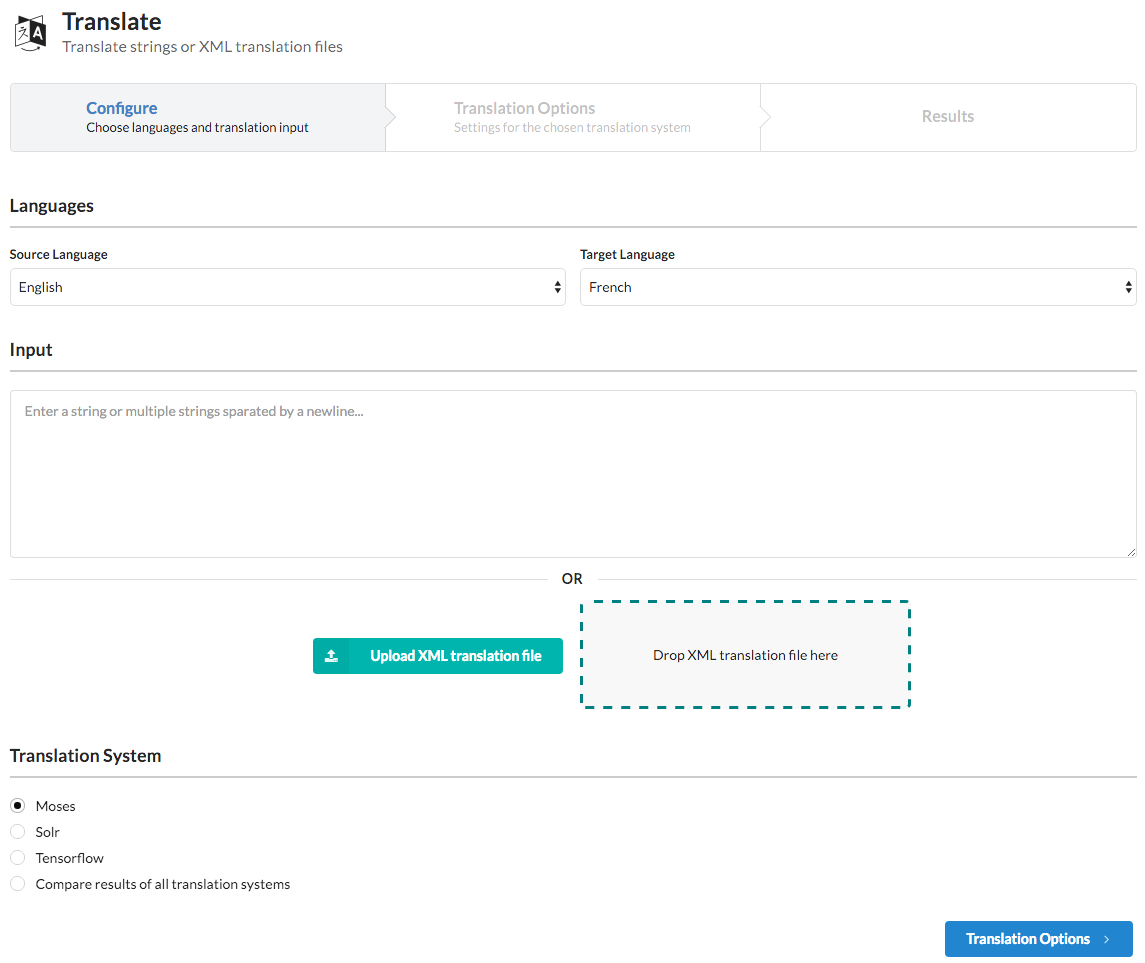
\includegraphics[width=0.9 \textwidth]{images/web_application_index.png}
    \caption[User interface of the web application]{First step to use the web application: Set source and target languages, translation input and choose the translation system.}
    \label{fig:web_app_index}
\end{figure}


\subsection{Translation Options}

\textbf{Moses}

\begin{itemize}
\item \textbf{Drop unknown words} Words not in the vocabulary are either dropped or replaced by the word in the source language. [No]
\item \textbf{Verbose} Verbosity level of the debug output. [2]
\item \textbf{Stack size} Number of hypotheses kept on each stack while decoding. [100]
\item \textbf{Tune weights manually} If enabled, the four weights for the translation model can be set manually (see Section \ref{subsec:moses_tuning}). Normally, the optimal weights from the tuning process are used. [No]
\end{itemize}
\textbf{Baseline System (Solr)}

\begin{itemize}
\item \textbf{Number of Rows} Number of rows returned by Solr when searching for a translation. [100]
\end{itemize}
\textbf{Tensorflow}

\begin{itemize}
\item \textbf{Number of Layers} Number of layers in the RNNs. [2]
\item \textbf{Size} Number of Cells in each layer. [256]
\end{itemize}
Note that the provided parameters must match a model that was trained with the same values, otherwise Tensorflow will fail to load the model.

\section{Architecture}

Each translation system implements a common interface (see UML in Figure \ref{fig:web_app_uml}). This makes it easy to support additional translation engines at any time.

\begin{figure}[H]
    \centering
    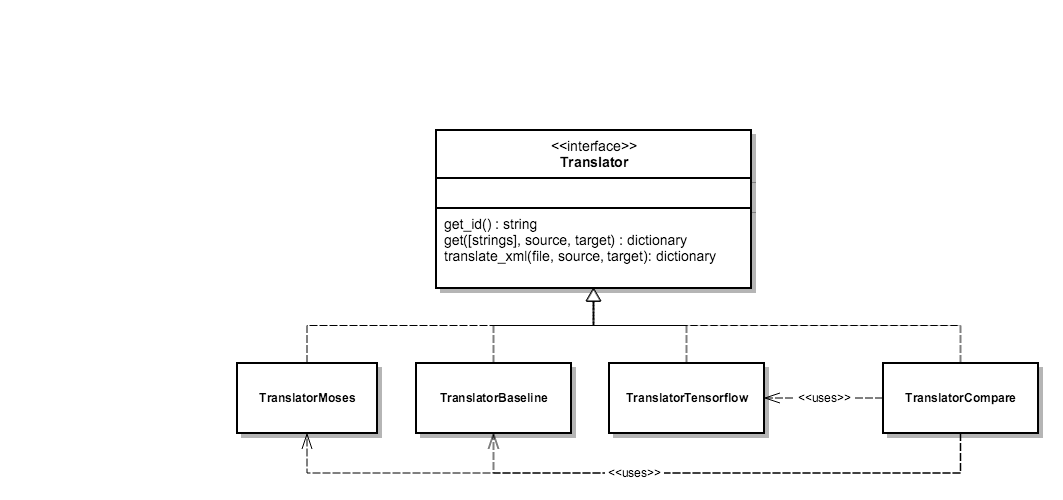
\includegraphics[width=1.0 \textwidth]{images/web_application_uml.png}
    \caption[UML diagram of the web application]{UML diagram: Each translation system implements the \emph{Translator} interface. The class \emph{TranslatorCompare} is special in a way that it gets the translations from all implemented systems, so that the results can be compared next to each other.}
    \label{fig:web_app_uml}
\end{figure}

The backend offers a REST based interface for the different functionalities. The frontend communicates through Ajax requests with that interface and handles the JSON responses accordingly.

\begin{figure}[H]
    \centering
    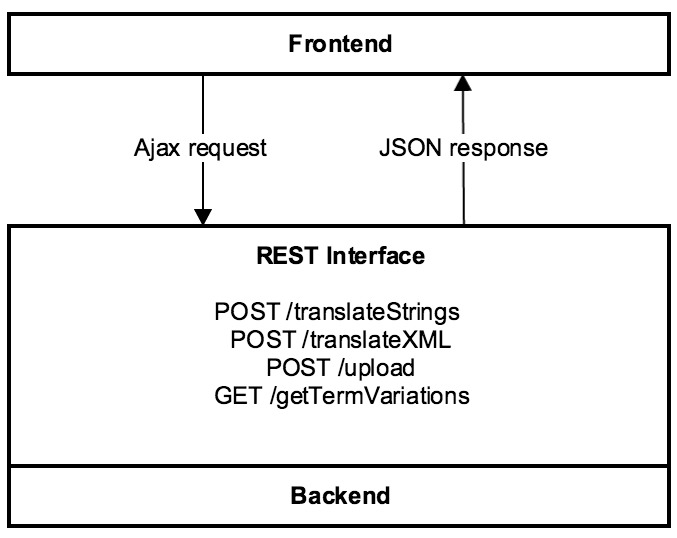
\includegraphics[width=0.5 \textwidth]{images/web_application_rest.png}
    \caption[REST interface]{The frontend communicates with the backend through a REST interface.}
    \label{fig:web_app_uml}
\end{figure}

The business logic is implemented in \emph{Python}, the REST interface is powered by a microframework called \emph{Flask}\footnote{\url{http://flask.pocoo.org/} (accessed: 16 May 2016)}. Flask has a built-in server and offers \emph{RESTful request dispatching}, among many other features. Table \ref{table_rest_endpoints} shows the possible endpoints of the REST interface together with the expected request data.

\begin{table}[H]
\centering
\begin{tabular}{@{}ll@{}}
\toprule
Endpoint                                                           & Request Data                                                                                                                                                                                                                                                                                  \\ \midrule
\begin{tabular}[c]{@{}l@{}}translateStrings \\ (POST)\end{tabular} & \begin{tabular}[c]{@{}l@{}}decoder: The ID of the translation system to use, e.g. ``moses''\\ decoder\_settings: JSON object of settings for the decoder\\ strings: Array of strings to translate\\ lang\_from: Source language code (e.g. ``en'')\\ lang\_to: Target language code (e.g. ``fr'')\end{tabular} \\ \midrule
\begin{tabular}[c]{@{}l@{}}translateXML\\ (POST)\end{tabular}      & \begin{tabular}[c]{@{}l@{}}decoder: The ID of the translation system to use\\ decoder\_settings: JSON object of settings for the decoder\\ xml\_filename: Hashed filename of the previous uploaded XML file\\ lang\_from: Source language code\\ lang\_to: Target language code\end{tabular}             \\ \midrule
\begin{tabular}[c]{@{}l@{}}getTermVariations\\ (GET)\end{tabular}  & \begin{tabular}[c]{@{}l@{}}source: Source language code\\ target: Target language code\\ term: String in source language\end{tabular}                                                                                                                                                         \\ \midrule
\begin{tabular}[c]{@{}l@{}}upload\\ (POST)\end{tabular}            & file: Data from uploaded XML translation file                                                                                                                                                                                                                                                 \\ \bottomrule
\end{tabular}
\caption{REST endpoints}
\label{table_rest_endpoints}
\end{table}

The frontend uses \emph{AngularJS}\footnote{\url{https://angularjs.org/} (accessed: 16 May 2016)} together with the \emph{Semantic UI}\footnote{\url{http://semantic-ui.com/} (accessed: 16 May 2016)} CSS framework.

% com.ancestry.android.apps.ancestry_your_capitalized
% com.google.android.apps.plus_collexion_abuse_appeal_rejected
% com.google.android.apps.plus_collexion_suspension_details
% --data_binary '{"id":"com.google.android.apps.plus_collexion_abuse_appeal_rejected","value":{"set":"votre"},"value_lc":{"set":"votre"}}'


\chapter{Evaluation}
\label{cha:evaluation}

How can we automatically measure the quality of machine translated text? There exists an algorithm called \emph{BLEU} \cite{bleu_score} which is mostly used for this task. We first shortly describe how BLEU works, then explain our evaluation setup and list the BLEU scores achieved for the different translation systems. Finally, we present the results of translating an existing app from English to French and German.

\section{BLEU (Bilingual Evaluation Understudy)}
\label{sec:bleu}

``The closer a machine translation is to a professional human translation, the better it is.'' This is the central idea behind the BLEU algorithm \citep{bleu_score}. BLEU computes a score by comparing machine translated sentences (called \emph{candiates}) against single or multiple reference translations. The score is averaged over the whole corpus to estimate the overall translation quality. The output of BLEU is a number between 0 and 1 that indicates the similarity of the candidate and reference translations. The closer a value is to 1, the more similar are the texts. %A value of 1 means that the candidate and reference translations are identical. 

\subsection{Algorithm}

BLEU compares \(n\)-grams of the candidate with \(n\)-grams of the reference translation and counts the number of matches. These matches are position-independent. The more the matches, the better the candidate translation is \cite{bleu_score}.

The score is based on a modified \(n\)-gram precision. One counts up the maximum number of times a \(n\)-gram occurs in any single reference translation. Next, one clips the total count of each candidate \(n\)-gram by its maximum reference count: \( count_{clip} = min(count, max\_ref\_count) \). The clipped counts for all \(n\)-grams are added up and divided by the total number of candidate words \citep{bleu_score}.
\\
\\
\textbf{Example} Consider this example from \cite{bleu_score} that computes a modified unigram precision:

\begin{itemize}
\item Candidate: \underline{the} \underline{the} the the the the the
\item Reference 1: \underline{The} cat is on \underline{the} mat.
\item Reference 2: There is a cat on the mat.
\end{itemize}
The word ``the'' appears twice in the first reference and once in the second reference, it is therefore clipped to:
\( count_{clip} = min(7, 2) = 2 \). The final modified unigram precision is \( P = \frac{2}{7} \).

To compute the modified precision score \(p_n\) for the entire corpus, we compute the \(n\)-gram matches for each sentence. Next, the clipped \(n\)-gram counts for all candidates are added up and divided by the number of candidate \(n\)-grams in the corpus:

\[  p_n = \frac{\sum_{C\in\{Candidates\}} \sum_{n-gram \in C} count_{clip}(n-gram)}{\sum_{C'\in\{Candidates\}} \sum_{n-gram' \in C'} count(n-gram')}   \]
In order to prevent very short candidates from receiving a too high  precision score, a \emph{brevity penalty} is introduced. This penalty is 1.0 if the candidate's length is the same as any reference translation's length. The closest reference sentence length is called \emph{best match length}. The brevity penalty is computed over the entire corpus. First, we compute the reference lengths \(r\) by summing the best match lengths for each candidate sentence in the corpus. We choose the brevity penalty to be a decaying exponential in \(r/c\), where \(c\) is the total length of the candidate translation corpus \cite{bleu_score}.

The final BLEU score is a combination of the brevity penalty \(PB\) and the geometric mean of the modified precision scores \(p_n\) of the corpus:

\[  BP = \begin{cases}1 & c > r\\e^{(1-\frac{r}{c})} & c \leq r\end{cases} \]

\[ BLEU = BP \: exp \left(  \sum_{n=1}^N w_n \:  log \: p_n \right) \]
The baseline in \citep{bleu_score} used \(N = 4 \) and uniform weights  \( w_n = 1/N \). 

\section{Setup}

The BLEU scores were computed in different evaluation runs for the results of translating English to French and German. We used \emph{k-fold cross-validation} to predict how the different models would perform if they were applied to independent data. The parallel corpus was split into 6 equal sized samples. One sample was always reserved as development set for Moses (Tuning) and Tensorflow, the remaining 5 samples were used to evaluate BLEU. For each evaluation run, four samples were merged into training data and a single sample was used as test set (see Figure \ref{fig:evaluation_k_fold}). One sample contains  19'158 parallel sentences for English-French and 19'129 sentences for English-German.

\begin{figure}[H]
    \centering
    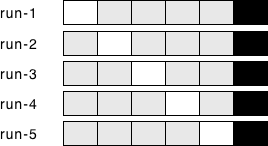
\includegraphics[width=0.4 \textwidth]{images/evaluation_k_fold_cross_validation.png}
    \caption[Evaluate BLEU score in different runs with k-fold cross validation]{Splitting the parallel corpus for multiple evaluation runs: The white rectangle represents the test data, grey means training data and the black rectangle is the fixed development sample.}
    \label{fig:evaluation_k_fold}
\end{figure}

The Baseline System needed a special setup. First of all, the development set is ignored since there is no evaluation or tuning involved in this model. Secondly, we needed to index the training data for each evaluation run separately into Solr. This was achieved by creating new cores in Solr according to the following schema:

\[ source-target-run-k-(source|target) \]
where \(source\) and \(target\) are the source and target language and \(k\) is the index of the evaluation run (1-5). For example, in the first evaluation run for translating English to French, the French training data is put into the core \texttt{en-fr-run-1-fr}.

\section{BLEU Scores}

A script\footnote{\url{https://github.com/moses-smt/mosesdecoder/blob/master/scripts/generic/multi-bleu.perl} (accessed: 16 May 2016)} included in Moses was used to compute the scores. As proposed in \citep{bleu_score}, \(n\)-grams up to \(n=4\) are considered in the calculation. Our corpus offers only one reference translation per sentence since apps are not translated multiple times into the same language. Note that the BLEU scores are reported as percentages, this format seems mostly used in machine translation literature. The left table shows BLEU scores achieved for translating English to French, the right one for English to German. The BLEU scores are reported for each evaluation run together with the average \(\o\) and standard deviation \(\sigma\).

\subsection{Moses}

\begin{table}[H]
\centering
\begin{minipage}{0.48\textwidth}
\centering
\begin{tabular}{@{}lrr@{}}
\toprule
EN-FR & BLEU\footnote{Language model using data from the monolingual corpus}  & BLEU\footnote{Language model using training data of each run}        \\ \midrule
run-1 & 47.45 & 43.11        \\
run-2 & 53.19 & 47.69        \\
run-3 & 49.91 & 44.23        \\
run-4 & 51.5  & 45.37        \\
run-5 & 51.74 & 46.31        \\
\textbf{\o}      & \textbf{50.76} & \textbf{45.34} \\
 \(\sigma\)     & 1.95   & 1.59        \\ \bottomrule
\end{tabular}
\label{my-label}
\end{minipage}
\hfill
\begin{minipage}{0.48\textwidth}
\centering
\begin{tabular}{@{}lrr@{}}
\toprule
EN-DE & BLEU\footnote{Language model using data from the monolingual corpus} & BLEU\footnote{Language model using training data of each run}         \\ \midrule
run-1 & 41.6 &  36.19       \\
run-2 & 44.53 & 40.37        \\
run-3 & 44.12  & 38.69       \\
run-4 & 46 & 39.09         \\
run-5 & 43.73 & 39.37        \\
\textbf{\o}      & \textbf{44.00} & \textbf{38.74}\\
 \(\sigma\)     & 1.42    & 1.39       \\ \bottomrule
\end{tabular}
\label{my-label}
\end{minipage}
\end{table}

The first column \emph{a} reports BLEU scores for a trained model where the language model uses all available data from the French/German monolingual corpus. This also includes sentences from the test sample, which might not be desired for a fair comparison. Hence, a second model was trained where the language model solely uses sentences from the French/German training corpus per run, not including sentences from the test sample. These BLEU scores are reported in the second column \emph{b}.

\subsection{Tensorflow}

\begin{table}[H]
\centering
\begin{minipage}{0.48\textwidth}
\centering
\begin{tabular}{@{}lrrrr@{}}
\toprule
EN-FR & BLEU\footnote{2 Layers, 256 Units, 40'000 words} &  BLEU\footnote{3 Layers, 512 Units, 40'000 words}     & BLEU\footnote{1 Layers, 128 Units, 40'000 words} & BLEU\footnote{2 Layers, 256 Units, 50'000 words} \\ \midrule
run-1 			& 19.86  			&   19.36			&	 23.13 			& 20.53     			\\
run-2 			& 26.7   			&   21.29    		&	25.68			& 22.44	\\
run-3 			& 25.27  			&   19.57    		&	23.2				& 21.07	\\
run-4 			& 20.64  			&   20.58    		&	20.48			& 26.86	\\
run-5 			& 27.43  			&   21.42  			&	22.21			& 28.49	\\
\textbf{\o}    	& \textbf{23.98} 	&  	\textbf{20.44}	&	\textbf{22.94}	& \textbf{23.88}	\\
 \(\sigma\)    	& 3.13           	&	0.85				&	1.68				& 3.2	\\ \bottomrule
\end{tabular}
\label{my-label}
\end{minipage}
\hfill
\begin{minipage}{0.48\textwidth}
\centering
\begin{tabular}{@{}lrrrr@{}}
\toprule
EN-DE & BLEU\footnote{2 Layers, 256 Units, 40'000 words} &  BLEU\footnote{3 Layers, 512 Units, 40'000 words}     & BLEU\footnote{1 Layers, 128 Units, 40'000 words} & BLEU\footnote{2 Layers, 256 Units, 50'000 words} \\ \midrule
run-1 			& 18.72  			&   18.58			&	20.02 			& 25.56     			\\
run-2 			& 23.95   			&   20.34    		&	19.93			& 24.13	\\
run-3 			& 22.14  			&   19.96    		&	22.04			& 23.62	\\
run-4 			& 19.66  			&   18.82    		&	19.86			& 26.87	\\
run-5 			& 17.03  			&   19.71  			&	20				& 24.11	\\
\textbf{\o}    	& \textbf{20.3} 	&  	\textbf{19.48}	&	\textbf{20.37}	& 	\textbf{24.86}	\\
 \(\sigma\)    	& 2.46           	&	0.67				&	0.84				& 1.2	\\ \bottomrule
\end{tabular}
\label{my-label}
\end{minipage}
\end{table}

\subsection{Baseline System}

\begin{table}[H]
\centering
\begin{minipage}{0.48\textwidth}
\centering
\begin{tabular}{@{}lr@{}}
\toprule
EN-FR & BLEU          \\ \midrule
run-1 & 25.08          \\
run-2 & 29.28          \\
run-3 & 25.35          \\
run-4 & 26.2           \\
run-5 & 25.7          \\
\textbf{\o}      & \textbf{26.32} \\
 \(\sigma\)     & 1.53           \\ \bottomrule
\end{tabular}
\label{my-label}
\end{minipage}
\hfill
\begin{minipage}{0.48\textwidth}
\centering
\begin{tabular}{@{}lr@{}}
\toprule
EN-DE & BLEU          \\ \midrule
run-1 & 8.74          \\
run-2 & 9.57          \\
run-3 & 9.03          \\
run-4 & 9.68           \\
run-5 & 8.98          \\
\textbf{\o}      & \textbf{9.2} \\
 \(\sigma\)     & 0.36           \\ \bottomrule
\end{tabular}
\label{my-label}
\end{minipage}
\end{table}


\subsection{Observations}

One can see that Moses produces the best translations according to the BLEU metric. As expected, if the language model component of Moses has less data available, the scores drop about 5 units. Still, the achieved BLEU scores are doubled compared to Tensorflow and the Baseline System. While deep learning neural networks achieve a slightly higher BLEU score than phrase based systems in \cite{smt_deep_learning}, this does not apply to our context. One reason probably is that our corpus is too small. In machine translation literature, the translation models are usually trained on much more data. The parallel corpus English-French from the \emph{European Parliament Proceedings Parallel Corpus} \cite{website_parallel_corpus} contains over 2 million sentences, which means \texttildelow 105 times more sentences than our corpus holds. Other than that, Moses has the advantage that its phrase table contains all possible words, while in Tensorflow, there is a fixed limit of the vocabulary size. Compared to Moses, Tensorflow also lacks of a tuning process, where the optimal model parameters are determined.

Surprisingly, increasing the model parameters in Tensorflow (add more layers and units to the network) did not improve translation quality. We achieved the best results with 2 layers and 256 units. Using 3 layers and 1204 units reduces the standard deviation though. Increasing the vocabulary size to 50'000 words did improve the BLEU score only for translating English to German.

The Baseline System produces similar results as Tensorflow for the translations from English to French. However, BLEU score is very low for translations from English to German. The reason is that the grammar of English and German is very different. Most sentences in English follow the \emph{Subject-Verb-Object} (SVO) syntax, which is not the case for German sentences. ``In German, the main verb must be the second element in the independent clause. This often requires an inversion of subject and verb''\footnote{\url{http://esl.fis.edu/grammar/langdiff/german.htm} (accessed: 16 May 2016)}. The Baseline System simply translates substrings without reordering, so \(n\)-grams in the candidate won't match with \(n\)-grams in the reference sentence. While the BLEU score for unigrams is reasonable, bigrams, trigrams and 4-grams do not contribute much to the overall BLEU score. The French grammar also follows the SVO syntax, which explains the better results for the translations from English-French.


\section{Translating existing app ``Farplano''}
\label{sec:translating_farplano}

BLEU represents the quality of translations with a single number, which is useful to quickly and automatically compare translation results. However, it is hard to imagine how the translations of a given BLEU score actually looks like. In this section, we are going to translate the app  \emph{Farplano}\footnote{\url{https://play.google.com/store/apps/details?id=com.schedulr} (accessed 25 May 2016)} from Roman Prokofyev, who supervised this thesis. Farplano displays public transport departures for the stations close to you in Switzerland.

As the app is already translated to French and German, the BLEU score can be computed as well. The following tables show a subset of the produced translations for translating the app from English to French and German. The third column \emph{Truth} shows the reference translation.

\begin{table}[H]
\centering
\def\arraystretch{1.25}
\begin{tabular}{@{}p{4.5cm}p{4.5cm}p{4.5cm}@{}}
\toprule
Source                                                                  & Translation                                                                       & Truth                                                                   \\ \midrule
Voice search                                                            & lors de la voix                                                                   & Recherche vocale                                                        \\
Manage subscriptions                                                    & G\'{e}rer les abonnements                                                             & G\'{e}rer les inscriptions                                                  \\
Search                                                                  & recherche                                                                         & Rechercher                                                              \\
Navigate home                                                           & Navigate d ' accueil                                                              & Revenir \`{a} l'accueil                                                     \\
Invalid Account                                                         & compte non valide                                                                 & Compte erron\'{e}                                                           \\
Share with                                                              & partager avec                                                                     & Partager avec                                                           \\
Show on the map                                                         & afficher sur la carte                                                             & Voir sur la carte                                                       \\
Set location                                                            & choisir le lieu                                                                   & R\'{e}gler la localisation                                                  \\
More options                                                            & plus d' options                                                                   & Plus d'options                                                          \\
Show buses                                                              & montrer les buses                                                                 & Montrer les bus                                                         \\
Buy ticket SMS                                                          & acheter des SMS de r\'{e}duction                                                      & Acheter billet SMS                                                      \\
Show trains                                                             & afficher des trains                                                               & Montrer les trains                                                      \\
min. connection duration                                                & dur\'{e}e de la connexion h min .                                                     & min. dur\'{e}e des correspondances                                          \\
Updating stationboard                                                   & la mise \`{a} jour stationboard                                                       & r\'{e}actualisation de horaire                                              \\
Failed to send message                                                  & \'{e}chec de l' envoi du message                                                      & Impossible d'envoyer le message                                         \\
Update location                                                         & mise \`{a} jour de l ' emplacement                                                    & R\'{e}actualiser de location                                                \\
Journey to …                                                            & Journey \`{a} …                                                                       & Voyage vers …                                                           \\
Cannot obtain location                                                  & Cannot obtenir la localisation                                                    & Ne peut pas obtenir une location                                        \\
Swipe up to start navigation to the current station                     & Glissez vers le haut pour d\'{e}marrer la station au courant                          & Glisser vers le haut pour commencer l'itin\'{e}raire vers l'arret actuel    \\
If you enjoy using FarPlano, would you mind taking a moment to rate it? & si vous aimez utiliser FarPlano, pourriez-vous prendre un moment pour \'{e}valuer it? & Si tu aimes utiliser FarPlano, peux-tu prendre un moment pour le noter? \\
Network Error                                                           & erreur réseau                                                                     & Erreur r\'{e}seau                                                           \\
Location services disabled                                              & les services de localisation d\'{e}sactiv\'{e}s                                           & Services de localisation d\'{e}sactiv\'{e}s                                     \\ \bottomrule
\end{tabular}
\caption{Results for translating Farplano from English to French.}
\label{table_farplano_en_fr}
\end{table}


% Please add the following required packages to your document preamble:
% \usepackage{booktabs}
\begin{table}[H]
\centering
\def\arraystretch{1.25}
\begin{tabular}{@{}p{4.5cm}p{4.5cm}p{4.5cm}@{}}
\toprule
Source                                                                  & Translation                                                                                  & Truth                                                                        \\ \midrule
Voice search                                                            & Voice suchen                                                                                 & Sprachsuche                                                                  \\
Manage subscriptions                                                    & Abonnements verwalten                                                                        & Abonnemente verwalten                                                        \\
Search                                                                  & Suche                                                                                        & Suchen                                                                       \\
Navigate home                                                           & Navigate home                                                                                & Zur Startseite                                                               \\
Invalid Account                                                         & Konto ung\"{u}ltig                                                                               & Ung\"{u}ltiges Konto                                                             \\
Share with                                                              & teilen mit                                                                                   & Freigeben für                                                                \\
Show on the map                                                         & auf der Karte anzeigen                                                                       & Auf der Karte zeigen                                                         \\
Set location                                                            & Ort :                                                                                        & Standort wählen                                                              \\
More options                                                            & weitere Optionen                                                                             & Weitere Optionen                                                             \\
Show buses                                                              & buses anzeigen                                                                               & Bussen anzeigen                                                              \\
Buy ticket SMS                                                          & SMS Ticket kaufen                                                                            & Billett kaufen SMS                                                           \\
Show trains                                                             & trains anzeigen                                                                              & Z\"{u}ge anzeigen                                                                \\
min. connection duration                                                & Dauer min .                                                                                  & min. Verbindungsdauer                                                        \\
Updating stationboard                                                   & stationboard aktualisieren                                                                   & Fahrpl\"{a}ne aktualisieren                                                      \\
Failed to send message                                                  & Nachricht senden an fehlgeschlagen                                                           & Nachricht konnte nicht gesendet werden                                       \\
Update location                                                         & Standort \"{a}ndern                                                                              & Ort aktualisieren                                                            \\
Journey to …                                                            & Journey zu …                                                                                 & Reise nach …                                                                 \\
Cannot obtain location                                                  & Standort Cannot erhalten                                                                     & Kann nicht Ort erhalten                                                      \\
Swipe up to start navigation to the current station                     & die Navigation starten Zieh den aktuellen Sender                                             & \emph{missing}                                                                         \\
If you enjoy using FarPlano, would you mind taking a moment to rate it? & wenn du gerne verwendest FarPlano, w\"{u}rdest du dir einen Moment Zeit , um uns zu bewerten it? & Sollte Dir FarPlano Spaß machen, macht es Dir etwas aus die App zu bewerten? \\
Network Error                                                           & es gibt ein Problem mit dem Netzwerk                                                         & Netzwerkfehler                                                               \\
Location services disabled                                              & Standort ist deaktiviert                                                                     & Standortdienste deaktiviert                                                  \\ \bottomrule
\end{tabular}
\caption{Results for translating Farplano from English to German.}
\label{table_farplano_en_de}
\end{table}


% 114948 total sentences in parallel corpus EN-FR
% http://esl.fis.edu/grammar/langdiff/german.htm
% https://en.wikipedia.org/wiki/Subject%E2%80%93verb%E2%80%93object
% https://de.wikipedia.org/wiki/Subjekt-Verb-Objekt
% http://esl.fis.edu/grammar/langdiff/french.htm

\chapter{Conclusion}

The question if it is possible to provide high-quality translations for apps with machine learning can be answered with ``Yes''. Still, one might argue that this answer depends on the definition of \emph{high-quality}. On one hand, we achieved good BLEU scores with a phrase-based system, as shown in Chapter \ref{cha:evaluation}. The achieved BLEU scores for Moses are higher than the scores achieved in \cite{smt_phrase_based, smt_deep_learning} on the \emph{European Parliament parallel corpus} \cite{website_parallel_corpus}, though the context is different, so a direct comparison is not possible. However, it still proofs our initial claim: Based on existing data and the similarity of sentences among different apps, we achieved a reasonable quality for machine translated sentences.  %that the concept of using existing data to translate new apps works. 
On the other hand, machine translated text is almost never perfect. Bad app translations can do more harm than good, users might get confused if they cannot understand the content. Because of that, machine translated text \emph{should} be reviewed and corrected or completed by humans.

Is there a market for a system proposed in this thesis? Maybe, but there is also the question how legal it is from a laws point of view. The \emph{terms of service} from the Google Playstore include the following paragraph: ``You may not sell, rent, lease, redistribute, broadcast, transmit, communicate, modify, sublicense or transfer or assign any Content or your rights to Content to any third party without authorization, including with regard to any downloads of Content that you may obtain through Google Play. Use of any tool or feature provided as an authorized part of Google Play (for example, ``Social Recommendations'') shall not violate this provision so long as you use the tool as specifically permitted and only in the exact manner specified and enabled by Google.'' \footnote{\url{https://play.google.com/intl/en_ch/about/play-terms.html} (Accessed: 16 May 2016)} According to this quotation, authorization would be necessary to use existing content, which might also include the translation data.


\section{Future Work}


The current state of the project could be improved in many ways. Currently, all available translations are used to train the SMT models, which also includes wrong or bad translations. We could rate translations based on metadata of the app they are coming from, e.g. number of downloads, average rating, number of ratings ect. In general, the more existing high-quality translations we collect to train the SMT models, the better the quality of our produced translations is.

Another possibility is to analyse what kind of sentences are translated well on which system. With this knowledge in mind, we could choose the optimal system based on the input sentence.

Lastly, the prototype web application could be improved as well. After translating an XML file, we could offer to download the results as XML file again, among other formats. An interesting option could be to connect the web application with a crowdsourcing service, where the produced translations can be corrected and extended by people from a community.


%END Doc
%-------------------------------------------------------

\bibliography{thesis}
\bibliographystyle{plain}


\begin{appendices}
\chapter{Source Code}
The complete source code is available on GitHub:
\\
\url{https://github.com/wanze/AppTranslator}
\end{appendices}


\end{document}
